\documentclass[12,twoside]{mammeTFM}
%\usepackage[active]{srcltx}
\usepackage{amsthm} % To make environments with different styles.
\usepackage{amsmath,amssymb,amsfonts} % Multiple mathematics symbols and fonts.
%\usepackage{amscd} % To make commutative diagrams
\usepackage{graphicx} % To include figures in a simple way. Fancy options can be found for example in http://www.kwasan.kyoto-u.ac.jp/solarb6/usinggraphicx.pdf
\usepackage{enumerate} % It allows you to make list with specific somehow arbitrary labels, like this one.
%\usepackage[all]{xy} % To make really fancy commutative diagrams
\usepackage{booktabs} % To make fancy tables.
%\usepackage[usenames]{xcolor}
%\usepackage{fancyhdr}

%%%%% My packages (Should probably push all the header to a certain file and include it in each latex.

%\usepackage[left=15mm, right=15mm]{geometry}
\usepackage[utf8]{inputenc}
\usepackage[english]{babel}
\usepackage{bigfoot}
%\usepackage{algorithm}
%\usepackage[noend]{algpseudocode}
\usepackage{epstopdf}
\usepackage{vhistory}
\usepackage{framed}
\usepackage{hyperref}
\usepackage{cancel}
\usepackage{subcaption}

\setlength{\parskip}{11pt}

% Theorem Environments: add extra ones at the end if you need it.
\newtheorem*{thmA}{Theorem A}
\newtheorem{thm}{Theorem}[section]

\newtheorem{prop}[thm]{Proposition}
\newtheorem{lem}[thm]{Lemma}
\newtheorem{cor}[thm]{Corollary}
\newtheorem{conj}[thm]{Conjecture}

\theoremstyle{definition}
\newtheorem{definition}[thm]{Definition}
\newtheorem{exmp}[thm]{Example}

\theoremstyle{remark}
\newtheorem{remark}[thm]{Remark}
\newtheorem*{remarknonumber}{Remark}
\newtheorem{observation}[thm]{Observation}
%%% My own theorems
\newtheorem{main_thm}[thm]{Main Theorem}

%% rme, rmi e Id son el número e, el número imaginario i y la identidad respectivamente. Poned ds antes de una expresión
%% cuando salga mal (en las fracciones y cosas parecidas)
\def\ds{\displaystyle}
\def\rme{\mathrm{e}}
\def\rmi{\mathrm{i}}
\def\Id{\mathrm{Id}}
\def\resposta{\bullet\bullet\bullet\bullet\bullet\bullet}

%%%%%%%%%%%%%%%%%%
% macros/abbreviations: Include here your own.
%%%%%%%%%%%%%%%%%%

%% Conjuntos típicos.
\newcommand{\N}{\ensuremath{\mathbb{N}}}
\newcommand{\E}{\ensuremath{\mathbb{E}}}
\newcommand{\Z}{\ensuremath{\mathbb{Z}}}
\newcommand{\Q}{\ensuremath{\mathbb{Q}}}
\newcommand{\R}{\ensuremath{\mathbb{R}}}
\newcommand{\C}{\ensuremath{\mathbb{C}}}
\newcommand{\F}{\ensuremath{\mathbb{F}}}
\newcommand{\MP}{\ensuremath{\mathbb{P}}}

% math stuff
\newcommand{\Expect}{\ensuremath{{\rm I\kern-.3em E}}}
\newcommand{\Var}{\ensuremath{\mathrm{Var}}}
\newcommand{\Cov}{\ensuremath{\mathrm{Cov}}}

% random
\makeatletter
\newcommand{\raisemath}[1]{\mathpalette{\raisem@th{#1}}}
\newcommand{\raisem@th}[3]{\raisebox{#1}{$#2#3$}}
\makeatother

\newcommand{\function}[5]{\begin{align*} #1\colon #2 &\to #3 \\ #4 &\mapsto #5\end{align*}}
\newcommand{\vega}{\nu}

%% Separacio correcta paraules final de linia.
\hyphenation{Bar-ce-lo-na}

%% Ejemplo de como hacer una tabla.

%\begin{tabular}{|r|c|c|}
%\hline
%$n$	&nº bits (estándar)	&nº bits (\emph{sp. triplet})\\
%\hline
%10   	  &  6400       	& 3040\\
%\hline
%50   	  & 160000    	& 78400\\
%\hline
%100 	  & 640000    	& 314320\\
%\hline
%200 	  & 2560000  	& 1262320\\
%\hline
%400 	  & 10240000	&5043680\\
%\hline
%650 	  & 27040000	&13282720\\
%\hline
%1000 	  & 64000000	&31479040\\
%\hline
%\end{tabular}


%% Ejemplo de como hacer una figura

%\begin{figure}[ht]
%\centering
%\includegraphics[width=6cm,angle=-90]{exemple.eps}
%\caption{Corba de continuaci\'o d'$u_2$ com a funci\'o de $\lambda$.}
%\label{fig:etiqueta}
%\end{figure} 

%% se puede hacer \input{archivo.tex} en lugar de \includegraphics

%% Y de como hacerle referencia

% bla bla bla en la Figura~\ref{fig:etiqueta}


% Body of document

\titol{Extension Of The SWIFT \\[3mm] Option Pricing Scheme \\[3mm] For European Options Calibration \\[3mm] Under Heston Stochastic Volatility Model}
\titolcurt{Heston Calibration using SWIFT}
\authorStudent{Eudald Romo Grau}
\supervisors{Luis Ortiz-Gracia}
\monthYear{June, 2020}

%\msc[2010]{Primary  	55M25, 57P10, Secondary 55P15, 57R19, 57N15.}

\paraulesclau{Options Trading, Heston, SWIFT, Calibration, Inverse Fourier Option Valuation}
\agraiments{
Thanks to...}


\abstracteng{A Heston model calibration technique is presented for European options under the Heston model. The novel Shannon Wavelets Inverse Fourier Technique (SWIFT) is expanded for European option price calibration (previously it was used only for pricing European, barrier, and bermudan options). This method has different expressions and speed-up techniques, adequate to different set-ups. These are discussed and new expressions and properties are presented for the gradient computation and option calibration.

The Heston characteristic function expression recently proposed by Cui et al. is used in the SWIFT implementation due to its analytic gradient and its continuity properties.

The performance, robustness, and convergence under real-market values is studied for different implementations of the SWIFT technique and compared with the option calibration scheme presented by Cui et al.

The SWIFT implementations are coded in C++ and uploaded to a public GitHub repository. The libray implements several of the different SWIFT expressions for GBM and Heston European options.
}

%%%%%%%%%
\begin{document}

\maketitle

\tableofcontents

\pagebreak

% The expected structure is explained in https://bibliotecnica.upc.edu/estudiants/6-passos-que-teu-tfg/tfm-sigui-exit/escric-meu-tfg/tfm#criteris-grafics

\section{Motivation}

Option pricing has an important role in contract trading, both as a form of derivative trading in itself, as well a way to hedge other stock or derivative portfolios.

Pricing these options can have a broad range of difficulty, mainly due to two factors:
\begin{enumerate}
\item \textbf{Contract type:} These options can take a variety of forms, from the relatively simple European Options to more complex American, Bermudan, or Asian options (see chapter \ref{chapter:option_valuation}).
\item \textbf{Underlying Model: } The price of the derivative depends on the future price of its underlying. The evolution of this price can be modeled using simpler models like Black \& Scholes (BS), which has an analytic closed form for European option pricing but fails to capture some key properties of real markets (see section \ref{subsec:bs}), or using more complex models like the Heston model (chapter \ref{chap:heston_model}) or L\'evy models other than BS (chapter \ref{chapter:levy}).
\end{enumerate}

Closed option price formulas only exist for European options under the BS model. Either using more complex option contracts or models generally means one must fall back to numeric schemes to obtain option prices, which typically means less robustness to numerical errors and more computational time.

Some of these pricing techniques rely on the fact that most of the well-known models have a characteristic function with a closed form and use that characteristic function to price options through risk-neutral option valuation techniques (see section \ref{subsec:riks_neutral} for an introduction to risk-neutral markets and section \ref{subsec:european_option_valuation} for its applications toward European option valuation). Recently one of these characteristic-function-based pricing methods, called Shannon Wavelets Inverse Fourier Technique (SWIFT) \cite{Ortiz-Gracia2016} has been shown to successfully price European, Barrier, and Bermudan options \cite{mar17} with models with closed-form characteristic function.

One does not have the choice of always pricing options as European contracts, as the type of contract is decided by the Contract Exchanges that trade derivative contracts, and even if one were to trade only European options, the study of more complex underlying price models is relevant, as BS fails to capture well-known properties of real markets, which is reflected in the implied volatility surface (see section \ref{subsec:smile_and_surf}), which option traders will to take into account if they use the BS mode. This motivated the development other models, like the stochastic volatility Heston model, which will be the main model considered for option price calibration in this study.

Calibration refers to finding values for the underlying model intrisic parameters that minimize the difference between real market option prices and the prices obtained through the model being calibrated (see chapter \ref{chap:optimization_problem} for the specific optimization problem considered in this study and how to solve it). As the real market option prices are constantly changing it is of special relevance to find calibration schedules that are highly time-efficient to allow real-time model updates.

In particular, the Heston model calibration is a difficult optimization problem to solve efficiently, as it is a multidimensional optimization problem with a fairly unknown structure (it is not known whether it is a convex problem or not nor whether it generally has a single solution or not) which until recently did not have simple analytic expressions for its characteristic function gradient \cite{cui17} (the implications of not knowing the problem structure and of not having simple analytic expressions for the gradient are discussed in section \ref{subsec:calibration_difficulties}.

The goal of this study is to extend the SWIFT method to calibrate complex option underlying models. In particular, the base European option pricing SWIFT method will be extended for European options under the Heston model expressions provided by Cui et al. \cite{cui17}. Then the performance of the resulting option calibration scheme will be compared against Cui's calibration technique. This calibration technique could then be extended to Barrier and Bermudan contracts following Maree et al. \cite{mar17} but will not be implemented here.

In order to extend SWIFT for calibration, an expression of the SWIFT price gradient is provided (see section \ref{subsec:gradient}) which can benefit from several performance speed-up techniques. Some of these techniques were already presented in \cite{Ortiz-Gracia2016} and \cite{mar17} and some are new to this study and are particularly useful for the SWIFT calibration to be competitive with other highly efficient calibration techniques like Cui's. To ensure this performance competitivity several speed and robustness test are presented (see chapters \ref{chapter:study}, \ref{chapter:results}).

\section{Option Valuation}\label{chapter:option_valuation}

\begin{definition}
An European Option is a derivative contract on an underlying asset that fixes a transaction price (called strike price), an expiration time (also called maturity), and an underlying asset quantity and gives the holder of the contract the right (but not the obligation) of buying (Call Option) or selling (Put Option) the specified quantity of the underlying at the Strike price on expiration.
\end{definition}

In the following sections we will use the following nomenclature for Option parameters: $t$ will refer to the time at which the option is being valuated and $T$ will be the expiration time. Given a time-dependent variable $V$, $V_t$ will refer to the value of that variable at time $t$ (respectively with $T$). $S, K$ will refer to the underlying and the strike prices respectively.

Slight variations of these terms can give rise to other families of options by facilitating the exercising of the contracts, like the Bermudan and American options (which allow to exercise your buying/selling right at specified instants of time or at any point prior to expiry, respectively).

Other groups of option families are obtained by changing the definition of the option payoff, that is, the amount of money (be it in cash or in the value of the underlying obtained) the option gives on expiration.

\begin{definition} Payoff of a Call European option:
\begin{equation} \label{eq:european_call_payoff}
V_{EC}(S_T, 0) = (S_T - K)\boldsymbol{1}_{S_T \geq K} = \left\{ \begin{array}{rcl}
S_T - K & \mbox{if} & S_T > K \\ 
0 & \mbox{if} & S_T\leq K
\end{array}\right.
\end{equation} 
\end{definition}

So, on maturity, a European Call option is only profitable if it allows the holder of the contract to buy the underlying asset at a cheaper price than the current asset spot price. In most models any option has a certain positive value if it's not expired, as the underlying price can always theoretically move enough so that a currently non-profitable option ends up with a positive payoff on expiry. Thus, one can always divide the price of an option with positive time to expiry $\tau$ as $V(S,\tau) = V_1(S) + V_2(S, \tau)$, where $V_1(S) := V(S,0)$ and is called the implicit value of the option, and $V_2(S, \tau)$ is its time value. The implicit value of an option is typically used to classify options as follows:

\begin{definition} A European option at time $t$ is called:
\begin{itemize}
\item {Out of the money (OTM):} If it has no implied value and exercising it would result in loss (that is $K > S_t$ for Call options).
\item {At the money (ATM):} If its implied value is 0 and exercising it would result in breaking even (that is $K = S_t$).
\item {In the money (ITM):} If it has positive implied value (that is, $K < S_t$ for Call options).
\end{itemize}

\end{definition}

Some examples of other families of functions that have different payoffs are Binary Options (only have two possible payoffs dependent on $K$ and $S_T$) and Asian Options (the payoff depends on the mean price of the underlying since the start of the contract and until maturity).

In order to price an option that expires at some point in the future, one usually first models the temporal evolution of the price of its underlying asset by using some stochastic process. This model will typically be expressed in terms of parameters that will be calibrated to fit the underlying price evolution of each product one wants to valuate.
% TODO: Some discussion on how the nature of the contract affects the difficulty of pricing it.

When pricing options, a risk-neutrality assumption is usually taken \cite{hul09}. In order to describe and justify this assumption, let's first look at the no-arbitrage assumption.

\subsection{No-arbitrage Assumption and Risk-neutral Markets}\label{subsec:riks_neutral}

Consider an option call contract C with strike K and current price $V_t$. Let the underlying associated with it have an initial price $S_t$ and maturity $\tau$, and model the underlying price evolution as a 1-step discrete process that follows a Bernouilli distribution, so that the final price of the underlying is:
\begin{definition}
\begin{equation}
S_T^{Ber} := \left\{ \begin{array}{rcl} u \cdot S_t & \mbox{with probability} & p_u \\
 d \cdot S_t & \mbox{with probability} & p_d := 1 -p \end{array}\right.
\end{equation}
\end{definition}

Once the underlying moves either up or down and reaches maturity, the price of the option will be determined by the the payoff formula $V(S_T, 0)$ given in \ref{eq:european_call_payoff}. The reasoning that will be followed in this section will apply to any type of option contract, so let's simply call these option values $V_u$ and $V_d$ respectively.

Then, one can hold a portfolio with a long position in the underlying and a short position in the options with ratio $n:1$, so that the value of the portfolio at time T is $n S_T - V(S_T, 0)$, and choose n so that the portfolio has the same value whether the underlying goes up or down by setting:
\begin{equation}
n S_t u - V_u = n S_t d - V_d \rightarrow n = \dfrac{V_u - V_d}{S_t(u - d)}
\end{equation}

This portfolio is what is called a risk-free portfolio, as its final value is perfectly defined and, if one assumes there are no arbitrage opportunities, its rate of returns must match the risk-free rate (which will be denoted r). Here, r rate denotes a theoretic rate at which one can earn money with almost no risk (in US markets is usually assumed to be the US-treasury bonds rate of return for the length of the considered invesment), and an arbitrage oportunity is the possibility to invest without risk obtaining a rate of returns higher than r (this can happen, for example, when a share is traded at two different markets, and the offers are different enough between the markets that one can buy a share in one market and sell it immediately in the other for a profit).

Its easy to see that if the rate of returns of the portfolio is different than r, arbitrage opportunities will arise. Let the values of the portfolio at times t and T be $P_t$ and $P_T$ respectively:
\begin{itemize}
\item If $P_T > P_t e^{r\tau}$: Anyone can start holding the porfolio or increase the volume they hold until expiry.
\item If $P_T < P_t e^{r\tau}$: Anyone who holds shares of the portfolio can sell them and invest the obtained cash without risk.
\end{itemize}

Hence, the no-arbitrage assumption provides a way to valuate the current price of an option through its expected payoff. One first needs to build a risk less portfolio and compute its expected payoff under a certain underlying price evolution model. Then one can discount the risk free rate during the maturity of the option contract to obtain the initial price of the portfolio and, from there, obtain the price of the option. That is:
\begin{lem} The price of a 1-step option under a Bernouilli model is
\begin{equation}
V(S_t, \tau) := e^{-r\tau} \left( p_u V_u + p_d V_d \right)
\end{equation}
\begin{proof}
First, from the portfolio initial value one can obtain $V(S_t, \tau) := n S_t - P_t$, as the portfolio is risk-less,  it earns the risk-free rate, so 
\begin{equation}
V(S_t, \tau) = n S_t - e^{-r\tau} P_T = n S_t - e^{-r\tau}\left(n S_t u - V_u \right) = nS_t(1 - u e^{-r\tau}) + V_u e^{-r\tau}
\end{equation}
Using the value of n for a risk-less portfolio, one obtains
\begin{align}
V(S_t, \tau) =& \dfrac{V_u - V_d}{S_t(u - d)} S_t(1 - u e^{-r\tau}) + V_u e^{-r\tau} \\
 =& \dfrac{V_u (1 - u e^{-r\tau}) - V_d (1 - u e^{-r\tau})}{(u - d)} + V_u e^{-r\tau} \\
 =& \dfrac{V_u (1 - d e^{-r\tau}) + V_d (u e^{-r\tau} - 1)}{(u - d)} \\
 \label{eq:discounted_expected_payoff}
 =& e^{-r\tau} \left( V_u P + V_d (1 - P) \right)
\end{align}
, where
\begin{equation}
P = \dfrac{e^{r\tau} - d}{u - d}
\end{equation}
\end{proof}
\end{lem}

Note that the price of the option is independent of $p_u$ and $p_d$. This probability is already taken into account in the price of the underlying and is a key concept of the modelization of real markets as risk-neutral ones. On the other hand, equation \ref{eq:discounted_expected_payoff} can be interpreted as the discounted expected payoff of the option, if its payoff were to follow a Bernouilli distribution with parameter P. This distribution is called the risk-neutral distribution of the option, and is the basis of risk-neutral option valuation.

The assumption of no-arbitrage is usually generalized when pricing options by the concept of risk-neutrality. A risk-neutral world has two main features that simplify the pricing of derivatives:
\begin{itemize}
\item The expected return on a stock (or any other investment) is the risk-free rate.
\item The discount rate used for the expected payoff on an option is the risk-free rate.
\end{itemize}

Hull discusses in depth the no-arbitrage and risk-neutrality assumptions in chapter 12 of \cite{hul09}, as well as providing several justifications as to why a risk-neutrality assumption is useful to provide prices for real market options.

\begin{remark}
A well-known consequence of the risk-neutrality assumption is the Put-Call parity equation:
\begin{equation}\label{eq:put_call_parity}
C - P = S_t - e^{-r\tau} \cdot K
\end{equation}
, where C and P are the prices of a European put and call contract, (Note that this equation is independent of the model used for the time evolution of the underlying). This provides a way to convert any European call pricing schemes presented in this study to European put ones and vice-versa. Refer to \cite{hul09} for a proof of equation \ref{eq:put_call_parity}.
\end{remark}

\subsection{European Option Valuation} \label{subsec:european_option_valuation}
The payoff of some option contracts, like Bermudan, Asian or American options, depends on the price of the underlying asset at several points in time, or even through all its life. European options payoff, on the other hand, only depends on the final price of the underlying asset on the moment of expiration of the contract ($S_T$). 

A general pricing formula for this kind of options uses the risk-neutrality assumption to compute the option price as the discounted expectation of the payoff at expiry. Then the pricing problem is equivalent to defining an stochastic process describing $S_T$ conditioned to the initial value $S_t$. If one considers generic stochastic variables x and y that fully describe the stochastic variables $S_t$ and $S_T$ respectively, the general pricing formula becomes:
\begin{equation}
\label{eq:integral_option_valuation}
v(x, \tau)  = e^{-r \tau}\E^{\Q}(v(y, 0)|x)  = e^{-r\tau} \int_{\R}v(y,0)f(y|x)dy)
\end{equation}
, where v denotes the option value, r the risk-neutral interest rate, $\E^{\Q}$ the expectation under the risk-neutral assumption.

Any choice of x and y will allow computing the value of the option through a numerical integration scheme, but most common underlying price models used for option pricing have simpler expressions in the log space, so a common choice when solving this expression is to define:
\begin{align}
\label{eq:y}
y = ln \left(\dfrac{S_T}{K} \right) \\
\label{eq:x}
x = ln \left(\dfrac{S_t}{K} \right)
\end{align}

Given this maturity state variable choice, one can express the payoff of a European put option as
\begin{equation} \label{eq:european_payoff}
v_{K}(y, 0) := K \cdot (1 - e^y)^{+} := K \cdot max(1 - e^y, 0)
\end{equation}
This expression has a lineal dependency with the strike of the option, so one can define the strike-free payoff:
\begin{equation}
g(y) := (1 - e^y)^{+} = \dfrac{v_{K}(y, 0)}{K}
\end{equation}

\begin{remark}
When solving equation \ref{eq:integral_option_valuation} using numerical methods, one should prefer calculating the price of a call option via the price of a put one with the same strike and apply the put-call parity formula to recover the original call price, as $e^y$ can have arbitrarily large values inside the integration domain which can lead to errors due to floating point arithmetics \cite{mar17}.
\end{remark}

There is a broad literature in methods to solve this integration problem for basic underlying asset models. Some of them, as Black and Scholes (BS), even have closed solutions (as will be seen in section \ref{subsec:bs}) but it is common that, for more complex models, $f(y|x)$ doesn't have a known expression.

In some cases, this can be circumvented by using numerical integration methods based on Fourier transforms, if there is a known expression for the characteristic function of $f(y|x)$
\begin{equation}
\hat{f}_y(u;x) = \int_{\R} f(y | x) e^{-iux} du
\end{equation}

This is the case of the L\'evi models and the Heston model which will be presented in the following sections.

\section{L\'evy Processes}\label{chapter:levy}
Some well known underlying asset log returns theoretical stochastic processes, as the Geometric Brownian Motion (GBM) model (known as the Black-Scholes-Merton\cite{bs73, mer73} model), can be considered inside a more general concept called L\'evy processes.

\begin{definition} A stochastic process $X = \{X_t : t \geq 0\}$ is considered a L\'evy process if:
\begin{itemize}
\item $X_0 = 0$ almost surely.
\item For any $0 \leq t_1 \leq t_2 \leq \cdots \leq t_n \leq \infty$, $X_{t_2} - X_{t_1}, X_{t_3} - X{t_2}, \cdots X{t_n} - X_{t_{n-1}}$ are independent.
\item $\forall s < t$, $X_t - X_s$ is equal in distribution to $X_{t-s}$
\end{itemize}
\end{definition}

A famous property of L\'evy processes is the L\'evy-Khintchine formula:
\begin{lem}\label{levy_khin} Let $X = (X_t)_{t\geq 0}$ be a L\'evy process. Then its characteristic function $Char_X(u)$ is:
$$
Char_X(u)(t) := \E \left[e^{i\theta X(t)}\right] = e^{t\left(aiu - \dfrac{\sigma^2 u^2}{2} + \int_{\{0\}^c}(e^{iu x} \textbf{I}_{|x| < 1})\Pi(dx)\right)} = e^{\psi_L(w)}
$$
, where $\psi_L(u)$ is called the characteristic L\'evy exponent, and $a \in \R$, $\sigma \geq 0$, and $\Pi$ is the L\'evy measure of X, a $\sigma$-finite measure satisfying $\int_{\{0\} ^c}(1 \wedge x^2)\Pi (dx) < \infty$
\end{lem}

Note that any L\'evy process can be completely characterized by the triplet $(a, \sigma, \Pi)$, which represent a linear drift, a Brownian motion, and a L'evy jump process respectively.

L'evy models in option pricing typically consider x and y as in expressions \ref{eq:x} and \ref{eq:y} and let $X_t := x$, $X_T := y$, and model the log returns evolution by a L'evy process. Then $\hat{f}(y|x) = \hat{f}(X_T|X_t)$ can be obtained through formula \ref{levy_khin}:
\begin{equation}\label{eq:levy_char}
\hat{f}_{y}(u; x) := 
\E\left[e^{iu X_T}\right] = 
\E\left[e^{iu (X_t + X_{T-t})}\right] = 
e^{-iu x}e^{-i u \mu_L T + T \psi_L(-u)} = 
e^{-iu x}\hat{f}(u) = 
\hat{f}_{y - x}(u)
\end{equation}

, where $\mu_L:= r - \psi_L(-i)$ is a drift correction term and $\psi_L(u)$is the characteristic L\'evy exponent of the underlying log-returns process.

\subsection{Black-Scholes-Merton Model} \label{subsec:bs}

A particular case of L\'evi processes is the widely used BS model, originally presented in \cite{bs73} by using the following stochastic differential equation:
\begin{definition} BS model price equation:
\begin{equation}
dS_t = \mu S_t + \sigma S_t W_t
\end{equation}
, where $W_t$ is a Brownian Motion process, $\sigma$ is called the BS volatility, and $\mu$ describes the drift of the underlying log returns and is usually considered $\mu = r$ for divident-free products.
\end{definition}

This model assumes the underlying process $S_t$ follows a lognormal distribution with standard deviation $\sigma$ and, for European options, equation \ref{eq:integral_option_valuation} can be solved analytically, obtaining the well-known BS valuation formula:

\begin{lem} \textbf{Black-Scholes-Merton valuation formula for European Call Options}:
\begin{align}
  C_K(\sigma; S_t, \tau) &= N(d_1)S_t - N(d_2) PV(K) \\
     d_1 &= \frac{1}{\sigma\sqrt{\tau}}\left[\ln\left(\frac{S_t}{K}\right) + \left(r + \frac{\sigma^2}{2}\right)(\tau)\right] \\
     d_2 &= d_1 - \sigma\sqrt{\tau} \\
PV(K) &=Ke^{-r\tau}
\end{align}
\end{lem}

The characteristic function $\hat{f}(u)$ can be obtained by setting $\psi_L (u) = -\dfrac{\sigma^2}{2}u^2$ in equation \ref{eq:levy_char} resulting in:
\begin{definition} \textbf{BS characteristic function:}
\begin{equation}
\hat{f}_{BS}(u) = exp{\left(-iu \left( r-q - \dfrac{1}{2}\sigma^2 \right) \tau - \dfrac{\sigma^2 u^2 \tau}{2} \right)}
\end{equation}
\end{definition}

\subsection{Implied Volatility smile and surface} \label{subsec:smile_and_surf}
If the GBM process modeled accurately real market prices, the BS model could be calibrated using several strikes to obtain a single implied volatility value, and that value would be a good estimator of the standard deviation of the historical standard deviation of the lognormal distribution of the underlying returns (which is called the historical BS volatility). This volatility could then be used to price any option of a given strike and maturity. 

In real markets, if one chooses a fixed expiry and calibrates a set  m different models using m different strikes $\{K_i\}$, the obtained implied volatilities $\{\sigma_i\}$ will probably differ. Further, if one estimates the historical volatility $\sigma_H$ from the historical log-returns, the obtained value may not coincide with any of the obtained implied volatilities.

If one were to plot the implied $\sigma_i$ over $K_i$, one would obtain a result similar to the ones in Figure \ref{fig:smile}, but the exact shape would depend on the underlying (and change over time). This strike evolution is traditionally called volatily smile (though it can have different names depending on the shape it takes, like volatility skew for equity markets).

There are several justifications as to why such smiles exist. Some of them involve limitations in the GBM description of the underlying stock returns, but some appeared after significant events, like the volatility skew in equity option markets, which only appeared after the stock market crash of 1987 \cite{hul09}. Their significance is better described with the concept of implied distribution.

If one assumes that the risk-neutrality and no-arbritage concepts hold true, then the real market option prices should follow from specifying a distribution function $f(y|x)$ and solving equation \ref{eq:integral_option_valuation}. One can then estimate the shape of the implied distribution $f(y|x)_I$ that would better match the option prices of a specific product and expiry (there are several techniques to do it, some described in \cite{jac96, pea00}). As can be seen in Figure \ref{fig:implied_distribution}, the upward trend in implied volatility for the deep ITM and OTM options in currency markets is translated into the implied distribution having fatter tails, and the upward trend for small strikes in equity markets translates into a distribution with higher stock market crash probabilities.

A similar effect happens when one fixes a strike price and computes its implied volatility over serveral expiries. The shape that results from plotting the implied volatility smile over time is called term structure and, when one plots the implied volatility over both strike price and time, one gets the so-called implied volatility surface.

The shape of the implied volatility surface holds certain information about the historical performances of the underlying. In particular, the distribution with fat tails implied by the currency market option prices describes the historical returns of the options underlying better than the GBM \cite{hul09}. This shows the inedequacies of the GBM model and the need for better theoretic descriptions of the underlying returns.

\begin{figure}
\centering
\begin{subfigure}{.5\textwidth}
  \centering
  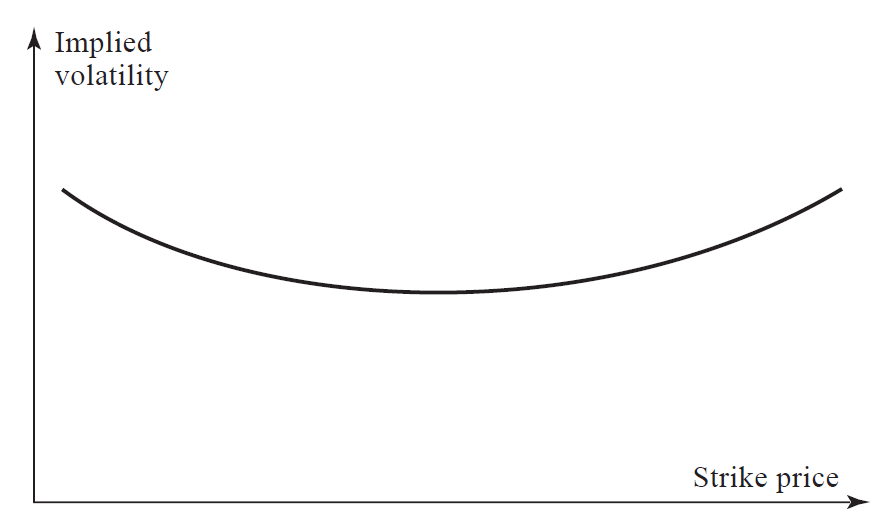
\includegraphics[width=.9\linewidth]{Media/currency_smile.PNG}
  \caption{Foreign Currency market.}
%  \label{fig:sub1}
\end{subfigure}%
\begin{subfigure}{.5\textwidth}
  \centering
  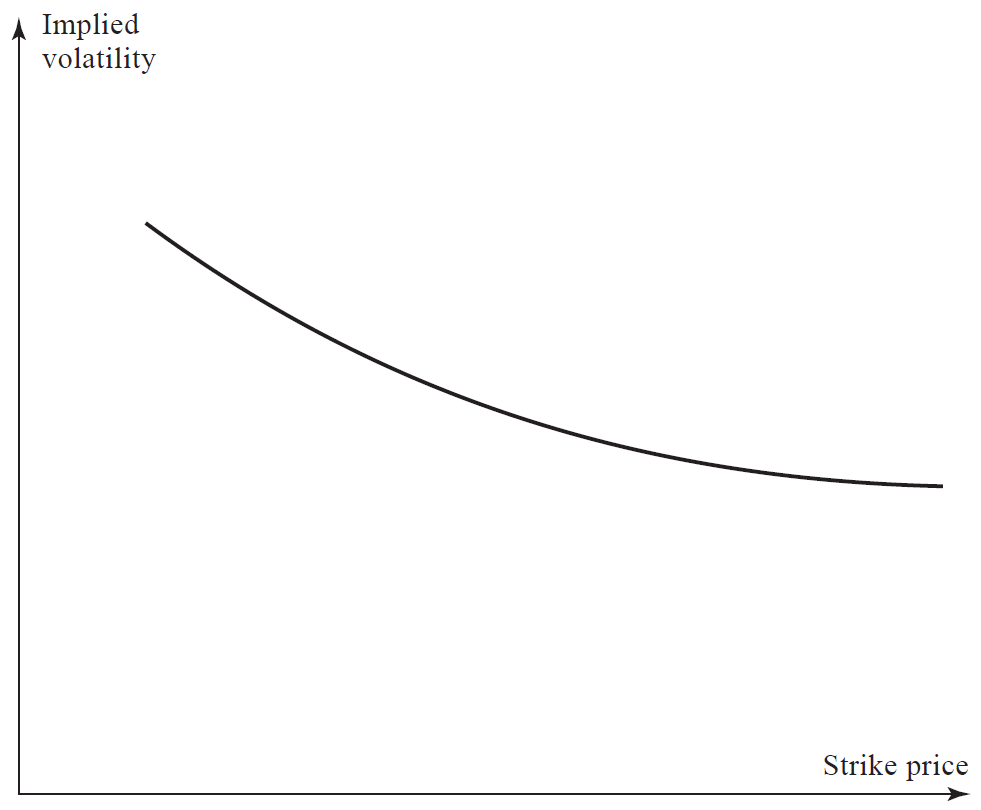
\includegraphics[width=.65\linewidth]{Media/equity_smile.PNG}
  \caption{Equity market.}
%  \label{fig:sub2}
\end{subfigure}
\caption{From \cite{hul09}. Volatility smiles for typical markets.}
\label{fig:smile}
\end{figure}


\begin{figure}
\centering
\begin{subfigure}{.5\textwidth}
  \centering
  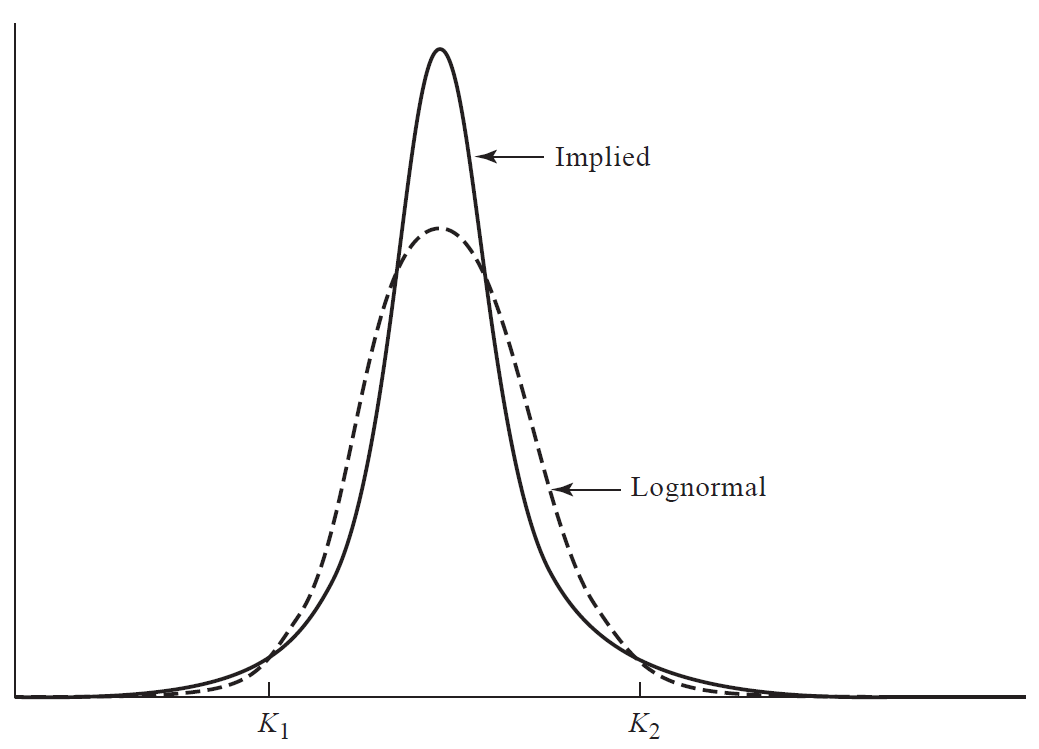
\includegraphics[width=.8\linewidth]{Media/currency_distribution.PNG}
  \caption{Foreign currency market}
%  \label{fig:sub1}
\end{subfigure}%
\begin{subfigure}{.5\textwidth}
  \centering
  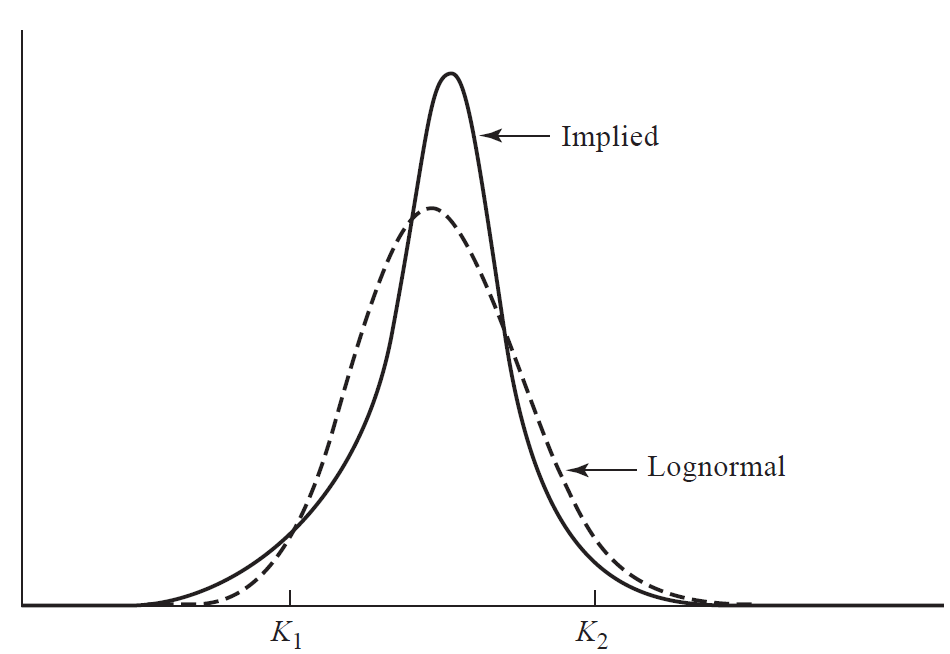
\includegraphics[width=.9\linewidth]{Media/equity_distribution.PNG}
  \caption{Equity market}
%  \label{fig:sub2}
\end{subfigure}
\caption{From \cite{hul09}. GBM (Lognormal) and Implied distributions for typical markets.}
\label{fig:implied_distribution}
\end{figure}

\section{Heston Model} \label{chap:heston_model}

The Black and Scholes model presented in section \ref{subsec:bs} fails to capture essential well-known properties of the real world market dynamics of the underlying return distributions, as its high kurtosis, its negative skew, the correlation between the underlying price and its volatility... As well as the risk premium investors give deep ITM or OTM options, which result in the volatility discussed in section \ref{subsec:smile_and_surf}.

To address that, several variations of this model have been proposed since it was introduced. Some of them, called stochastic volatility (SV) models, considered all the real world dynamics mentioned above and treated both the underlying price and its volatility as (potentially correlated) stochastic processes.

One of the first and most well-known SV models is the Heston model, defined by the following system of stochastic differential equations.

\begin{definition} Heston model price-volatility equations:
$$
dS_t = \mu S_t dt + \sqrt{\nu_t} S_t W_t^{(1)}
$$
$$
d\nu_t = \kappa(\overline{\nu} - \nu_t) dt + \sigma \sqrt{\nu_t}dW_t^{(2)}
$$
$$
dW_t^{(1)}dW_t^{(2)} = \rho dt
$$
, where $\nu_t$ is the variance of the underlying asset price at time t. The parameters $\kappa$, $\overline{\nu}, \sigma, \rho$ are respectively called: mean-reversion rate, long-term variance, volatility of volatility, and correlation between the Brownian processes $W_t^{(1)}$ and $W_t^{(2)}$. From now on, $\boldsymbol{\theta} := (\nu_0, \overline{\nu}, \rho, \kappa, \sigma)^T$ will refer to the vector of model parameters.
\end{definition}

Several studies have shown the relations between the Heston model parameters and the shape of the implied volatility surface \cite{cla11, gat06, gil12, jan11} necessary to obtain the same prices with a BS model. These relations can be summarized as follows:

\begin{itemize} \label{hes_param_properties}
\item $\nu_0$ controls the position of the volatility surface.
\item $\rho$ controls its skewness.
\item $\kappa$ and $\sigma$ control the convexity of the surface.
\item $\kappa(\nu_0 - \overline{\nu})$ controls the term structure of implied volatility.
\end{itemize}

Heston also provided an expression of the price of an European option, which will be adapted here in terms of the state variables x and y defined in section\ref{subsec:european_option_valuation}:

\begin{align} 
\label{eq:option_valuation_expectation}
& v(x, \tau) & = e^{-r \tau}\E^{\Q}(v(y, 0)|x) & = e^{-r \tau} \E^{Q}(K(e^y - 1)\boldsymbol{1}_{y \geq 0}) \\  
\label{eq:option_valuation_useless}
&  &  & = Ke^{-r \tau}(\E^{Q}(e^y \boldsymbol{1}_{y \geq 0}) - \E^{Q}(\boldsymbol{1}_{y \geq 0})) \\
\label{eq:option_valuation_final_form}
&  &  & = K e^x e^{-q \tau} P_1(\boldsymbol{\theta}; x, \tau) - K e^{-r \tau} P_2(\boldsymbol{\theta}; x, \tau)
\end{align}
, where $P_1$ and $P_2$ are defined as:
\begin{align}
&P_{1}(\boldsymbol{\theta} ; x, \tau)=\frac{1}{2}+\frac{1}{\pi} \int_{0}^{\infty} \operatorname{Re}\left(\frac{e^{i u x}}{i u} \frac{\hat{f}(\boldsymbol{\theta} ; -u+i, \tau)}{\hat{f}(\boldsymbol{\theta} ;i, \tau)}\right) \mathrm{d} u\\
&P_{2}(\boldsymbol{\theta} ; x, \tau)=\frac{1}{2}+\frac{1}{\pi} \int_{0}^{\infty} \operatorname{Re}\left(\frac{e^{iux}}{i u} \hat{f}(\boldsymbol{\theta} ; -u, \tau)\right) \mathrm{d} u
\end{align}
, where $\hat{f}$ is the characteristic function of the process followed by the logarithm of price of the underlying asset. The expression of this characteristic function is:
\begin{equation} \label{eq:char_heston}
\begin{aligned}
\hat{f}(\boldsymbol{\theta} ; u, \tau):=\mathrm{E}\left[\exp \left(-i u \log \frac{S_{T}}{S_{t}}\right)\right]=\exp \left\{i u r \tau\right.
\left.\quad+\frac{\kappa \bar{v}}{\sigma^{2}}\left[(\xi+d) \tau-2 \log \frac{1-g_{1} e^{d \tau}}{1-g_{1}}\right]+\frac{v_{0}}{\sigma^{2}}(\xi+d) \frac{1-e^{d \tau}}{1-g_{1} e^{d \tau}}\right\}
\end{aligned}
\end{equation}
, where

\noindent\begin{minipage}{.3\linewidth}
\begin{equation}
\xi:=\kappa + \sigma \rho i u
\end{equation}
\end{minipage}
\noindent\begin{minipage}{.4\linewidth}
\begin{equation} \label{eq:char_d}
d:=\sqrt{\xi^{2}+\sigma^{2}\left(u^{2} - i u\right)}
\end{equation}
\end{minipage}
\noindent\begin{minipage}{.3\linewidth}
\begin{equation}
g_{1}:=\frac{\xi+d}{\xi-d}
\end{equation}
\end{minipage}

Substituting these values into equation \ref{eq:option_valuation_final_form}, one can obtain an analytic equation to obtain the price of European Call options. Here, the expression given in \cite{cui17} is adapted to the state variables x and y and provided in a more compact form (the dependence on $\boldsymbol{\theta}$ and $\tau$ is not displayed on $\hat{f}$ for readibility):

\begin{lem} Heston's pricing method.
\begin{equation} \label{eq:heston_analytic}
C(\theta ; K, \tau)= K \left[ \frac{1}{2}\left(e^x- e^{-r \tau}\right) 
 + \frac{e^{-r \tau}}{\pi}\int_{0}^{\infty} \operatorname{Re}\left( \frac{\hat{f}(-u+i; x) - \hat{f}(u; x)}{i u}\right) du\right]
\end{equation}
\begin{proof}
Directly adapting equation (9) from \cite{cui17} to the state variables used in this article (and assuming the dicscount rate q = 0, which we assume through all this study) yields:
\begin{equation}
\begin{aligned}
C(\theta ; K, \tau)= \frac{1}{2}\left(S_{t}-K e^{-r \tau}\right) + \frac{e^{-r \tau}}{\pi}& \left[  S_t \int_{0}^{\infty} \operatorname{Re}\left(\frac{e^{i u x}}{i u} \hat{f}(-u+i)\right) \mathrm{d} u\right. \\
&\left.- K \int_{0}^{\infty} \operatorname{Re}\left(\frac{e^{i u x}}{i u} \hat{f}(-u)\right) du\right]
\end{aligned}
\end{equation}
. Dividing and multiplying everything by K, and using $S_t/K = e^{log(S_t/K)} = e^x$, one obtains
\begin{equation}
\begin{aligned}
C(\theta ; K, \tau)= K \frac{1}{2}\left(e^x- e^{-r \tau}\right) + K\frac{e^{-r \tau}}{\pi}& \left[\int_{0}^{\infty} \operatorname{Re}\left(\frac{e^{i (u - i) x}}{i u} \hat{f}(-u+i)\right) \mathrm{d} u\right. \\
&\left.- \int_{0}^{\infty} \operatorname{Re}\left(\frac{e^{i u x}}{i u} \hat{f}(u)\right) \mathrm{d} u\right]
\end{aligned}
\end{equation}
Joining the two integrals, and using the Heston characteristic function property $\hat{f}(u; x) = e^{-iu x}\hat{f}(u)$ one obtains the expression given in equation \ref{eq:heston_analytic}
\end{proof}
\end{lem}

From this expression, one can compute the analytic gradients of the option price in terms of the derivatives of the characteristic function. Then they can be used to optimize an appropriate objective function using gradient-descent based methods (See chapter \ref{chap:optimization_problem}) but, as will be explained in the next section, the analytic derivatives have not been widely used traditionally to calibrate Heston models prior to Cui et al. due to the complexity of the expressions obtained by derivating the available characteristic function expressions as eq \ref{eq:char_heston}  \cite{cui17}.

\subsection{Calibration Difficulties} \label{subsec:calibration_difficulties}
As opposed to simpler 1-dimensional models, Heston model calibrations is a multidimensional optimization problem with 5 degrees of freedom. Furthermore, the structure of this optimization problem is not known.

According to \cite{cui17} no consensus exists among researcher regarding whether the objective function of this optimization problem is convex or not. Some results point to a non-convex function, as the calibration methods proposed in \cite{che07, mik03} (which yielded different results for different initial points) and one must use long or short term approximations and rules to provide a sufficient initial guess. Recent research claims to provide methods that reach a unique solution independently of the initial point \cite{ger12} which, according to that study this indicates some structure that, even if not necessarily convex, tends to lead an initial guess to a stationary result.
There's also no consensus on whether the problem always has a single  optimum. In particular, it is known that there exists dependencies between the parameters that yield to similar results. For example, $lim_{t \rightarrow \infty} Var(\nu_t) = \dfrac{\sigma^2 \overline{\nu}}{\kappa}$, so large values of $\kappa$ and $\sigma$ can provide a model that prices options similarly to one with proportionally smaller values of these two parameters. The study by Cui et al. \cite{cui17} defends that this yields to the the objective function of the optimization problem flat close to the optimum.

As said above, there's no guarantee that a gradient-based method converges to the global optimum of the model parameters, but even obtaining a local optimum has been traditionally difficult. A lot of literature uses numerical gradients\cite{ger12} for these methods when trying to solve the Heston calibration problem (which are less accurate and more computationally consuming), because no simple analytic gradients were available and the ones obtained with symbolic algebra packages from the expressions of the characteristic function were intractable.

Prior to the work of Cui et al. \cite{cui17}, the existing methods could be summarized as:

\begin{itemize}
\item{\textbf{Heuristic based models:}}
Using the relationships stated in \ref{hes_param_properties}, some studies reduce the dimension of the optimization problem by assuming some values or relationships between the parameters from the observation of a specific volatility surface. For example, Gatheral sets $\nu_0$ to the short-term ATM implied variance obtained by using a BS model \cite{gat06}, an heuristic further justified by Chen \cite{che07}, where the linearity between $\nu_0$ and the BS implied volatility was verified for short maturities (less than 2 months). Other heuristics used in the industry are $\kappa = \dfrac{2.75}{\tau}$ and setting $\overline{\nu}$ to the BS short term volatility \cite{cla11}.

These assumptions may restrict the optimization problem domain and exclude the optimum.
\item{\textbf{Stochastic methods:}}
They are usually used in combination with deterministic search methods, as the Nelder and Mead simplex method \cite{lag98} and would avoid the pitfalls of the gradient-based methods if the optimization problem is not convex. Some examples are Wang-Landau \cite{che07}, differential evolution and particle swarm \cite{gil12_2}, and simulated annealing.
These methods are too computationally expensive for real-time use as of now: Fernandez et al. use GPU computations to calibrate options using a SV model called SABR, and it took 421.72 seconds to calibrate 12 instruments with tolerance of $10^{-2}$ using 2 NVIDIA Geforce GTX470 GPUs \cite{fer13}.

%\item{\textbf{Deterministic methods:}}

\end{itemize}

\subsection{Alternative Expressions}

For long-term maturities (i.e. big values of $\tau$), Kahl and J\"{a}ckel show that the characteristic  \ref{eq:char_heston} has discontinuities as $u$ increases \cite{kal06}, which can lead to numerical problems for many option valuation methods based on the integral expression \ref{eq:integral_option_valuation}. They show that this discontinuities arise because of a term in equation \ref{eq:char_heston} of the form $G^\alpha(u) := e^{\alpha log G(u)}$ with $G(u) := \dfrac{1 - g_1 e^{d\tau}}{1 - g_1}$ and $\alpha := \dfrac{\kappa \overline{\vega}}{\sigma^2}$, for non-integer values of $\alpha$. This is due to the spiral shape of $G(u)$ which produces a phase jump on $log(G(u))$ each time $G(u)$ crosses the negative side of the real line.

Albrecher et al. \cite{Albrecher2007} showed that the dicontinuity arises from taking the principal value of the square root in d (see equation \ref{eq:char_d}) and it can be avoided if the second value is used. In fact, it was proven that this alternative expression was continuous in the full parameters space \cite{sch04}

\begin{lem}
\begin{equation} \label{eq:char_schouten}
\hat{f}(\boldsymbol{\theta} ; u, \tau)=\exp \left\{-i u r \tau
+\frac{\kappa \bar{v}}{\sigma^{2}}\left[(\xi-d) \tau-2 \log \frac{1-g_{2} e^{-d \tau}}{1-g_{2}}\right]+\frac{v_{0}}{\sigma^{2}}(\xi-d) \frac{1-e^{-d \tau}}{1-g_{2} e^{-d \tau}}\right\} 
\end{equation}
, where $g_2 = \dfrac{1}{g_1}$
\end{lem}

A more compact version of the characteristic function was later derived by del Ba\~no Rollin et al. \cite{rol10} from the moment generating function of the process. This expression also had the benefit of replacing the u-dependent power functions in equations \ref{eq:char_heston} and \ref{eq:char_schouten} by hyperbolic functions, which greatly simplified obtaining analytic expressions of the gradient of the characteristic function.

\begin{lem}
\begin{equation} \label{eq:char_del_bano}
\hat{f}(\boldsymbol{\theta} ; u, \tau)=\exp \left(-i u r \tau + \frac{\kappa \bar{v} \rho \tau i u}{\sigma}-A\right) B^{2 \kappa \bar{v} / \sigma^{2}}
\end{equation}

, where
\begin{equation}\begin{array}{l}
A:=\frac{A_{1}}{A_{2}} \\
A_{1}:=\left(u^{2} - i u\right) \sinh \frac{d \tau}{2} \\
A_{2}:=\frac{d}{v_{0}} \cosh \frac{d \tau}{2}+\frac{\xi}{v_{0}} \sinh \frac{d \tau}{2} \\
B:=\frac{d e^{\kappa \tau / 2}}{v_{0} A_{2}}
\end{array}\end{equation}
\end{lem}

This last expression also showed discontinuity problems, as the original characteristic function in equation \ref{eq:char_heston}, but Cui, del Ba\~no Rollin, and Germano provided an equivalent expression, continuous in the full parameters domain, and with an analytic expression for its gradient.

\begin{thm}\label{theorem:cui} \textbf{Cui's expression of the Heston characteristic function.}
\begin{equation} \label{eq:char_cui}
\hat{f}(\boldsymbol{\theta}; u, \tau) = exp \left(-i u r \tau + \dfrac{\kappa \bar{v} \rho \tau i u}{\sigma}-A + \dfrac{2 \kappa \bar{v}}{\sigma^{2}}D \right)
\end{equation}
is an algebraically equivalent representation of equation \ref{eq:char_heston}, continuous through all the parameters space, where
\begin{equation}
D := \log \frac{d}{v_{0}}+\frac{(\kappa-d) \tau}{2}-\log \left(\frac{d+\xi}{2 v_{0}}+\frac{d-\xi}{2 v_{0}} e^{-d \tau}\right)
\end{equation}
. Further, its gradient with respect to the Heston model parameters $\boldsymbol{\theta} = (\nu_0, \overline{\nu}, \sigma, \kappa, \rho)^{T}$ is given by:
\begin{equation}
\nabla \hat{f}(\boldsymbol{\theta}; u, \tau) = \boldsymbol{h}(u) \hat{f}(\boldsymbol{\theta}; u, \tau)
\end{equation}
, where $\boldsymbol{h}(u) = [h_{v_0}(u), h_{\overline{v}}(u), h_\sigma(u), h_\kappa(u), h_\rho(u)]^T$ and:
\begin{align}
h_{v_0}(u)& =-\frac{A}{v_{0}} \\
h_{\overline{v}}(u)& =\frac{2 \kappa}{\sigma^{2}} D+\frac{\kappa \rho \tau i u}{\sigma} \\
h_{\sigma}(u)& =-\frac{\partial A}{\partial \rho}+\frac{2 \kappa \bar{v}}{\sigma^{2} d}\left(\frac{\partial d}{\partial \rho}-\frac{d}{A_{2}} \frac{\partial A_{2}}{\partial \rho}\right)+\frac{\kappa \bar{v} \tau i u}{\sigma} \\
h_{\kappa}(u)& =-\frac{1}{\sigma i u} \frac{\partial A}{\partial \rho}+\frac{2 \bar{v}}{\sigma^{2}} D+\frac{2 \kappa \bar{v}}{\sigma^{2} B} \frac{\partial B}{\partial \kappa}+\frac{\bar{v} \rho \tau i u}{\sigma} \\
h_{\rho}(u)& =-\frac{\partial A}{\partial \sigma}-\frac{4 \kappa \bar{v}}{\sigma^{3}} D+\frac{2 \kappa \bar{v}}{\sigma^{2} d}\left(\frac{\partial d}{\partial \sigma}-\frac{d}{A_{2}} \frac{\partial A_{2}}{\partial \sigma}\right)-\frac{\kappa \bar{v} \rho \tau i u}{\sigma^{2}}
\end{align}
, where the partial derivatives of A, $A_2$, B, and d are given in \cite{cui17} and can be seen in appendix \ref{app:cui_extra}
\end{thm}

%\subsection{Moment Generating Function} \label{subsec:heston_moment}

%In \cite{rol09}, the moment generating function for the Heston model is provided for the stochastic variable $X_t := ln(S_t) - \mu \tau$. Adapting it to provide it for $y|x$ one obtains:
%\begin{equation}
%\begin{aligned}
%M(u)=\mathbb{E}\left[ e^{u X_{t}}\right] = e^{- x u} exp & \left[ \dfrac{2 \kappa \overline{\nu}}{\sigma^{2}} \left( \dfrac{(\kappa-\sigma \rho u) \tau}{2} - log \left(cosh \left(\dfrac{P(u) \tau}{2} \right)+(\kappa-\sigma \rho u) \dfrac{sinh \left(\dfrac{P(u) \tau}{2} \right)}{P(u)}\right) \right) \right. \\
%& \left. -\mu \tau -v_{0} \dfrac{\left(u-u^{2}\right) \dfrac{sinh \left(\dfrac{P(u) \tau}{2} \right)}{P(u)}}{cosh \left(\dfrac{P(u) \tau}{2} \right)+(\kappa-\sigma \rho u) \dfrac{sinh \left(\dfrac{P(u) \tau}{2} \right)}{P(u)}} \right]
%\end{aligned}
%\end{equation}

%, where $P(u)=\sqrt{(\kappa -\rho \sigma u)^{2}+\sigma^{2}\left(u-u^{2}\right)}$

%This expression will be useful to bound the mass at the queues of the probability function $f(y|x)$.

%\begin{lem} \label{lem:my_lemma}
%\begin{equation}
%C(\boldsymbol{\theta}; K, \tau) = Ke^{-r\tau} \left[ \dfrac{e^x - 1}{2} + \dfrac{1}{\pi} \int_0^{\infty} Re \left( \dfrac{\hat{f}(u - i; x) - \hat{f}(u; x)}{iu} \right) du \right]
%\end{equation}
%\end{lem}

%\begin{lem} \label{lem:my_lemma_2}
%\begin{equation}
%C(\boldsymbol{\theta}; K, \tau) \approx C_1 :=  Ke^{-r\tau} \left[ \dfrac{e^x - 1}{2} + \dfrac{1}{\pi} \sum_{1 - \kappa}^{\kappa} D_{m,k} \int_0^{\infty} Re \left( \dfrac{\hat{\hat{f}}_{m,k}(u - i) - \hat{\hat{f}}_{m,k}(u)}{iu} \right) du \right]
%\end{equation}
%\end{lem}

\section{Multi Resolution Analysis and Shannon Wavelets}

\subsection{Multi Resolution Analysis} \label{def:mra}
Multi Resolution Analysis (MRA) is a method that ultimately allows to express any function in $L^2(\R)$ using a countable orthogonal family of wavelets. This family can then be truncated into a finite family and the original function can be orthogonally projected into the resulting subspace, obtaining an approximation with a certain level of resolution. Increasing the considered number of members of the wavelet family will increase the resolution of the approximation, converging to a perfect representation when all the wavelets are used \cite{tour}.

Given the space $L^2(\R) = \left\{f: \int_{-\infty}^{\infty}{|f(x)|^2 dx < \infty} \right\}$, a Multi Resolution Analysis is defined as 
a family of nested successive approximation closed spaces:
$$ \cdots \subset V_{-2} \subset V_{-1} \subset V_0 \subset V_1 \subset V_2 \subset \cdots $$

Where the subpsaces $V_i$ are complete (they are not redundant and cover $L^2(\R)$:
$$\overline{\bigcup_{i\in{\Z}}{V_i}} = L^2(\R) \text{, and } \bigcap_{m\in{\Z}} = {0}$$

, they have self-similarity in scale (all spaces are geometric scalings of $V_0$ by powers of 2):
$$ f(x) \in V_i \Leftrightarrow f(2x) \in V_{i + 1} $$

, they have self-similarity in time:
$$ f(x) \in V_0 \Rightarrow f(x - k) \in V_0, \forall k \in \Z $$

(Note that self-similarity in scale implies that the self-similarity in time translates to all spaces $V_i$ as $f(x) \in V_i \rightarrow f(x - 2^i k) \in V_i$.), and the integer shifts of a (or a finite group of) generator function $\phi$ form an orthogonal basis of $V_0$. 

In summary, we can define:

\begin{definition} \label{def:mra} (MRA): Consider $\phi \in L^2(\R)$ a wavelet that spans the family $\{\phi_{m,k}\}m,k\in\Z$ defined as the normalized scaled integer shifts of $\phi$. That is, $\phi_{m,k} = 2^{m/2}\phi(2^m x - k)$, and let $V_m := closure_{L^2(\R)}\left\langle\{\phi_{m,k}\}_{k \in \Z}\right\rangle$ 
\end{definition}

Then, if $\phi$ and $V_m$ fulfill the conditions above, we say that $\phi$ is the scaling function or father wavelet of the MRA $\{V_m\}$ (note that the previous definition properly defines $\{V_m\}$ as a sequence of nested subspaces and that $\phi$ provides an orthonormal basis for each of them).

One of the important implications of obtaining a father wavelet and its MRA is that another wavelet family can be obtained from it, which will be a basis of $L^2(\R)$. In order to do that, let's consider the set of subspaces $W_m$ such that $V_{m+1} = V_m \oplus W_m$. Then $L^2(\R) = \sum_m{\oplus W_m}$ and there exists a function $\psi \in W_0$ (called mother wavelet) that generates an orthonormal basis of $L^2(\R)$ \cite{dau92} by defining the wavelet functions:
$$ \psi_{m, k} = 2^{m/2}\psi(2^m x - k)$$
. Note that each $\{W_{m,k}\}_{k \in \Z}$ gives an orthonormal basis of $W_m$, and $\{W_{m_k}\}_{m\in [-\infty, m-1], k \in \Z}$ is an orthonormal basis of $V_m$. So for any $m \in \Z$ we can define 
\begin{definition} \label{def:wavelet_projection}
\textbf{Wavelet Projection:} $P_m: L^2(\R) \rightarrow V_m$ is the projection from any function $f \in L^2(\R)$ into $V_m$:
\begin{equation} 
P_m f(x) = \sum_{j = -\infty}^{m-1} \sum_{k \in \Z} d_{j,k} \psi_{j, k}(x) = \sum_{k \in \Z} D_{m,k} \phi_{m, k}(x)
\end{equation}

, where $d_{j, k} = \left\langle f,\psi_{j, k}\right\rangle$, $D_{m,k} = \left\langle f,\phi_{m, k}\right\rangle$, and $\left\langle f,g\right\rangle = \int_\R f(x) \overline{g(x)} dx$. Further, this projection converges in the $L^2$ norm as m tends to infinity \cite{tour}.
\end{definition}

\subsection{Shannon Wavelets}
Claude Shannon introduced the usage of the cardinal sine function for information modeling \cite{sha49}:
\begin{equation}
sinc(x) := \left\{ \begin{array}{rcl} \dfrac{sin(\pi x)}{\pi x} & \mbox{for} & x \neq 0 \\ 1 & \mbox{for} & x = 0 \end{array}\right.
\end{equation}

This function serves as the father wavelet from which we obtain the families $\phi_{m, k}$ and $\psi_{m_k}$:
\begin{equation}
\begin{array}{rcl}
\label{eq:wavelet}
\phi_{m,k}(x) = 2^{m/2} sinc(\pi (2^m x - k)), & k \in \Z
\end{array}
\end{equation}
\begin{equation}
\begin{array}{rcl}
\psi_{m,k}(x) = 2^{m/2} \left( sinc(\pi (2^m x - k - 1/2)) - \dfrac{sin(2 \pi (2^m x - k - 1/2))}{\pi (2^m x - k - 1/2)} \right), & k \in \Z
\end{array}
\end{equation}

One of the interesting properties of Shannon wavelets it that they have both a slow decay in time domain and a simple expression and sharp compact support in the frequency domain.
\begin{equation} \label{eq:sharp_freq}
\begin{array}{rcl}
\hat{\phi}_{m,k}(w) = \dfrac{e^{-i k/2^m w}}{2^{m/2}}rect \left(\dfrac{w}{2^{m+1}\pi}\right), & k \in \Z
\end{array}
\end{equation}
\begin{equation}
\begin{array}{rcl}
\hat{\psi}_{m,k}(w) = -\dfrac{e^{-i \dfrac{k + 1/2}{2^m} w}}{2^{m/2}} \left(rect \left(\dfrac{w}{2^{m}\pi} - \dfrac{3}{2}\right) + rect \left(-\dfrac{w}{2^{m}\pi} - \dfrac{3}{2}\right) \right), & k \in \Z
\end{array}
\end{equation}

When using Shannon Wavelets to approximate a function with a truncated wavelet expansion \cite{mar17} shows a bound for the projection error into $V_m$, by using concepts of band-limited functions:

\begin{definition} A function f is called band-limited if $\exists B \in \R^+$, with $B < \infty$ such that
\begin{equation}
f(x) = \dfrac{1}{2\pi} \int_{-B \pi}^{B \pi} \hat{f}(u) e^{iu x}du 
\end{equation}
, that is, the support of $\hat{f}$ is contained in the interval $[-B, B]$. The parameter B is referred to as the bandwidth of f.
\end{definition}

The nested subspaces of a Shannon MRA can be expressed in terms of band-limited functions because of the sinc Fourier transform rectangular shape, as stated in the following lemma from \cite{ste11}

\begin{lem} Consider an MRA generated from the Shannon scaling function as defined in \ref{def:mra}, then each subspace $V_m$ corresponds to the space of functions $f \in L^2(\R)$ with bandwidth $B \leq 2^m$
\end{lem}

Combining this lemma with the $L^2$ convergence of the projections $P_m$ of $f$ into $V_m$ yields the following corollary \cite{mar17}

\begin{cor} The orthogonal projection $P_m$ of a Shannon MRA is equivalent to:
\begin{equation}
P_m f(x) = \dfrac{1}{2 \pi} \int_{-2^m \pi}^{2^m \pi} \hat{f}(u) e^{i u x} d u
\end{equation}
\end{cor}

Which, in turn, can be used to derive the following bound to the error of the orthogonal projection.

\begin{definition}Given $f \in L^2(\R)$, let $H(\xi)$ be:
\begin{equation}
H(\xi) := \dfrac{1}{2 \pi} \int_{|u| > \xi}\left|\hat{f}(u)\right| du
\end{equation}
, the normalized mass of the two-side tails of $\hat{f}$ defined by $\xi$.
\end{definition}

\begin{lem} \label{lem:projection_error} Let $\epsilon_m(x) := f(x) - P_m f(x)$ (the pointwise approximation error due to the projection of f into $V_m$). Then $|\epsilon_m(x)| \leq H(2^m \pi)$ \cite{mar17}
\end{lem}


\subsection{Sinc Integral}\label{sec:sinc_integral}
Shannon MRA and SWIFT require solving integrals of the form $\int_{\R} f(x) g(sinc(x)) dx$. In particular, when one wants to compute the density coefficients $D_{m,k}$ of equation \ref{def:wavelet_projection}, or as will be seen in section \ref{subsec:payoff_coefficients}, for the payoff coefficients computation, one needs to solve integrals of the form $\int_{\R} f(x) \overline{\phi(x)} dx$ and $\int_{\R} f(x) \phi(x) dx$ respectively.

The simplest situation is to compute the sinc integral $Si(t) = \int_0^t{sinc(x) dx}$, but even for this case there is no closed form for the integral. 

There are two commonly used approaches as to how to numerically approximate these integrals, and their equivalency wa. 

\begin{itemize}
\item{ \textbf{Coefficients via Parseval's Theorem: } This approach, shown in \cite{ort16} uses the fact that the $\phi_{m,k}$ has a very small support in the frequency domain (as shown in equation \ref{eq:sharp_freq}) together with Parseval's theorem, 
$\langle f, g \rangle = \dfrac{1}{2 \pi}\langle \hat{f}, \hat{g} \rangle$. As the coefficients will be real numbers, we can take $\langle f, g \rangle = Re \left( \langle f, g \rangle \right) = Re \left( \dfrac{1}{2 \pi}\langle \hat{f}, \hat{g} \rangle \right)$. Entering the real part operator inside the integral sign and applying the change of variable $t = \dfrac{u}{2^{m+1} \pi}$ results in expression:
\begin{equation}
D_{m,k} = 2^{m/2} \int_{-1/2}^{1/2} Re \left(\hat{f}(2^{m+1} \pi t) e^{i2\pi k t} \right) dt
\end{equation} 
Any quadrature can be applied to numerically compute the integral, but there are known techniques to rearrange the trapezoid and midpoint quadratures to compute all the coefficients with a single FFT \cite{mar17, flo20}.
}
\item { \textbf{Coefficients via Sinc approximations: }
An equivalent expression of the sinc function was presented in \cite{Ortiz-Gracia2016} as a cosine expansion using Vieta's formula: 
\begin{equation}
sinc(x) = \prod_{j = 1}^{\infty} cos \left( \dfrac{\pi x}{r^j} \right)
\end{equation}
This cosine expansion was then truncated and converted to a summation via the cosine product-to-sum-identity
\begin{equation} \label{eq:density_v}
\prod_{j=1}^{\iota} \cos \left(\frac{\pi x}{2^{j}}\right)=\frac{1}{2^{\iota-1}} \sum_{j=1}^{2^{\iota-1}} \cos \left(\frac{2 j-1}{2^{\iota}} \pi x\right)
\end{equation}
obtaining the first expression for the vieta coefficients $D_{m,k}^v$, where
\begin{equation}
D_{m,k} \approx D_{m,k}^{v}= \frac{2^{m / 2}}{2^{\iota-1}} \sum_{j=1}^{2^{\iota-1}} \int_{\mathbb{R}} f(x) \cos \left(\frac{2 j-1}{2^{\iota}} \pi\left(2^{m} x-k\right)\right) d x
\end{equation} \label{eq:density_vc}
Finally, $f(x)$ would be replaced in the integral by defining $D_{m,k}^{v} = Re \left( D_{m,k}^{vc} \right)$. 
\begin{equation}
D_{m,k}^{vc} =  \dfrac{2^{m / 2}}{2^{\iota-1}} \sum_{j=1}^{2^{\iota-1}} \int_{\mathbb{R}} f(x) e^{-i\dfrac{2 j-1}{2^{\iota}} \pi\left(2^{m} x-k\right) } d x
\end{equation}
Notice that when applying the $Re(\cdot)$ operator to $D_{m,k}^{cv}$, it can move freely across multiplications by real numbers and sumations and integrals, and expression \ref{eq:density_v} is ultimately recovered by using $Re \left(e^{-uix}\right) = cos(x)$. Finally, splitting the complex exponential into x-dependent and x-independent terms and replacing $\int_{\R} f(x) e^{-xAi}$ by $\hat{f}(A)$ yields:
\begin{definition} \textbf{Vieta coefficients approximation}\label{def:vieta}
\begin{equation}
D_{m,k}^{*} =  \dfrac{2^{m / 2}}{2^{\iota-1}} \sum_{j=1}^{2^{\iota-1}} Re \left( \hat{f} \left(u_j 2^{m} \right) e^{ik u_j} \right)
\end{equation}
, where $u_j = \dfrac{\pi}{2^{\iota}}(2j - 1)$
\end{definition}
}
\end{itemize} 

It is worth noting that, while the original construction of expression \ref{def:vieta} required a sumation of a power of 2 number of terms, it was revisited in \cite{mar17} and generalized by expressing the sinc in terms of its Fourier transform 
\begin{equation}
sinc(t) = Re(sinc(t) = \dfrac{1}{2\pi} \int_{-\pi}^{\pi} Re \left( e^{-iux} du \right) = \dfrac{1}{\pi} \int_{0}^{\pi} cos(ux) du
\end{equation}
Then, if one uses a mid-point quadrature with J buckets and proceeds as in the initial derivation, expression \ref{def:vieta} is recovered, with the new term J being equivalent to the previous $2^{\iota -1}$ one.

The following approximation error bound was given in \cite{mar17} for the mid-point quadrature, which will be of special interest in section when analysing the approximation error of pricing an option with the SWIFT algorithm in section \ref{subsec:approximation_error}:

\begin{lem} \textbf{Error of the Sinc Function Approximation}
\begin{equation} \label{lem:error_sinc}
sinc^{*}(x; J) = \dfrac{1}{J}\sum_{j = 1}^J Re\left( e^{-iu_jx} \right)
\end{equation}
, where $u_j = \dfrac{\pi (2j - 1)}{2J}$. Then the approximation error of applying the midpoint quadrature on a finite domain $|x| \leq a \leq \dfrac{\pi}{2}J$ is bounded by:
\begin{equation}
max_{|x| \leq a} \left|sinc(x) - sinc^{*}(x; J) \right| \leq \dfrac{(\pi a)^2}{(4J)^2 - (\pi a)^2}
\end{equation}
\end{lem}

Note that this approximation only holds for a bounded interval of the sinc function domain. This implies that, when used to compute a sinc integral, the integral must also be truncated so that $|x| \leq \dfrac{\pi J}{2}$.

In particular, if one approximates the shannon wavelet $\phi_{m,k}(x)$ in the domain $(a, b)$ by using the $sinc^{*}(x;J_k)$, the sinc function will be evaluated in the domain $(2^m a - k, 2^m b - k)$ and one can obtain a bound on $J_k$ for each wavelet. A will be seen in section \ref{subsec:fft}, using a single value J that fulfills the unequality $max(|2^m a - k|, |2^m b - k|) \leq \dfrac{\pi J}{2}$ for all k will allow to speed up computations by using a Fast Fourier Transform algorithm. So, assuming a single value J is used and symmetric domains (-c, c) and $[1 - \kappa, \kappa]$ are considered for x and k respectively, one obtains the following corollary, presented in a slightly different form in \cite{mar17}:
\begin{cor} \textbf{Error of the Wavelet Approximation}
\begin{equation}
\phi_{m,k}^{*}(x) := 2^{m/2} sinc^{*}(2^m x -k; J)
\end{equation}
. Then the error of applying the midpoint quadrature on a finite domain $|x| \leq c$ for all $k \in [k1, k2]$ is (assuming a fixed $J \geq \dfrac{\pi}{2}(2^m c + \kappa)$) 
\begin{equation}
\max _{|y| \leq c, 1-\kappa \leq k \leq \kappa}\left|\phi_{m, k}(y)-\phi_{m, k}^{*}(y)\right| \leq 2^{\frac{m}{2}} \frac{\left(\pi\left(2^{m} c+\kappa\right)\right)^{2}}{(4 J)^{2}-\left(\pi\left(2^{m} c+\kappa\right)\right)^{2}}
\end{equation}
\end{cor}

%\section{Pricing by Gatheral}

\section{SWIFT} \label{chapter:swift}

The Shannon Wavelets Inverse Fourier Technique (SWIFT) combines the Shannon Wavelets and Multiresolution Analysis concepts with equation \ref{eq:integral_option_valuation} to provide a fast approximation to the value of a specific option v(x, t).

The overall approximation can be summarized, as in \cite{mar17}, by a set of consecutive approximation steps to that equation, which are described below. The error related to each of these approximations will be analyzed in section \ref{subsec:approximation_error}.

\begin{itemize} \label{swift_steps}

\item \textbf{Wavelet Projection:} f is substituted by its Shannon wavelet projection at scale $m \in \Z$. By lemma \ref{def:wavelet_projection} this can be stated as:
\begin{equation} \label{step:wavelet_projection}
f(y|x) \approx f_1(y|x) := P_mf(y|x) = \sum_{k \in \Z} D_{m,k}(x) \phi_{m,k}(y)
\end{equation}
\begin{equation}
v(x,t) \approx v_1(x,t) = e^{-r \tau} \int_{\R} f_1(y|x)v(y, T)dy
\end{equation}
, with $D_{m,k}(x):=\langle f(\cdot | x), \phi_{m,k} \rangle$
\item \textbf{Series Truncation: } The set of values of k partaking the sum \ref{step:wavelet_projection} is reduced to a finite interval $[k1, k2]$
\begin{equation}
f_1(y|x) \approx f_2(y|x) = \sum_{k = k1}^{k2} D_{m,k}(x)\phi_{m,k}(y)
\end{equation}
\begin{equation} \label{step:series_truncation}
v_1(x,t) \approx v_2(x,t) = e^{-r \tau} \int_{\R} f_2(y|x)v(y, T)dy
\end{equation}
It is important to notice that the first approximation lets us express: 
\begin{equation}
f(2^{-m}k|x) \approx f_1(2^{-m}k|x) = 2^{m/2} D_{m,k}(x)
\end{equation}
, which quickly justifies that, for any given x, the density coefficients vanish as $|k|$ increases, because f vanishes at the queues. It is also worth noting that increasing m will result in this mapping being less favorable. That is, for each k, $D_{m,k}$ will be bounded by a point closer to the center of the density function, potentially requiring to increase the interval $[k1, k2]$.
\begin{remark}
From this point onward a symmetric interval $[1 - \kappa, \kappa]$ will be considered both for convenience and for consistency with the code implementation.
\end{remark}
\item \textbf{Density Coefficients Approximation: }
The integral required to compute $D_{m,k}$ is replaced by an approximation $D_{m,k}^{*}$ as discussed in section \ref{sec:sinc_integral}.
\begin{equation}
f_2 (y|x) \approx f_3(y | x) = \sum_{k = 1 - \kappa}^{\kappa} D_{m,k}^{*}(x)\phi_{m,k}(y)
\end{equation}
\begin{equation}
\begin{aligned}
v_2(x,t) \approx v_3(x,t) & = e^{-r \tau} \int_{\R} f_3(y|x)v(y, T)dy \\
&= e^{-r \tau} \sum_{k = 1 - \kappa}^{\kappa} D_{m,k}^{*}(x)  V_{m,k}dy
\end{aligned}
\end{equation}
, where
\begin{equation}
V_{m,k} := \int_{\R} \phi_{m,k}(y) v(y, T)dy
\end{equation}
\item \textbf{Payoff Coefficients Approximation: }
The integral required to compute $V_{m,k}$ is approximated in an analogous way as the integral to compute the density coefficients.
\begin{equation}
v_3(x,t) \approx v_4(x,t) = e^{-r \tau} \sum_{k = 1 - \kappa}^{\kappa} D_{m,k}^{*}(x) V_{m,k}^{*}
\end{equation}

For European Put options the payoff is given by equation \ref{eq:european_payoff}, and the last equation can be rearranged using the strike-free payoff as

\begin{equation} \label{step:final}
v_4(x,t) = K e^{-r \tau} \sum_{k = 1 - \kappa}^{\kappa} D_{m,k}^{*}(x) U_{m,k}^{*}
\end{equation}
, where $U_{m,k}^{*}$ is the approximation of 
\begin{equation} \label{eq:compact_payoffs}
U_{m,k} := \int_{\R} \phi_{m,k}(y)g(y) dy = \int_{-\infty}^{0} \phi_{m,k}(y)(1-e^{y}) dy
\end{equation}

This coefficients can be precomputed when initializing the SWIFT procedure and shared across different strikes and maturities, saving computation time.
\begin{remark}
The approximation $D_{m,k}^{*}$ depends on a parameter J that represents the number of intervals in the sinc approximation quadrature. The parameter used for payoff computation is independent from the one used for the density coefficients, and will be labeled $J_p$ and $J_d$ respectively.
\end{remark}
\end{itemize}

\begin{remark}
This section and section \ref{subsec:approximation_error} follow closely section 3 of \cite{mar17}. There, the error analysis of the approximation process starts with a truncation of the integration space of equation  \ref{eq:integral_option_valuation}, for which an explicit error bound is not provided. Here, this error is accounted for in the payoff coefficients approximation step and its explicitly specified.
\end{remark}

\subsection{Payoff Coefficients Approximation} \label{subsec:payoff_coefficients}
One should note that the same procedure as the approximation $D_{m,k} \approx D_{m,k}^{*}$ (discussed in section \ref{sec:sinc_integral}) can be used for the payoff coefficients approximation. Starting from expression \ref{eq:compact_payoffs}, and applying the same sinc approximation as in the density coefficients, for european puts we obtain expression:

\begin{equation}
U_{m,k} \approx \dfrac{2^{m/2}}{J_p}\sum_{j=1}^{J_p} Re \left( e^{i \dfrac{2j - 1}{N_p} \pi k} \int_{\R} (1 - e^y)^{+} e^{-i \dfrac{2j - 1}{N_p} \pi y} \right)
\end{equation}

The last step of the density coefficients approximation requires the convergence of the Fourier transform of the payoff coefficients which, in general, is not guaranteed. In particular the Fourier transform of the strike-free payoff of an european put option does not converge.

The $sinc^{*}$ approximation is only defined in a finite domain anyway, so the SWIFT algorithm implementations deal with this situation by initially bounding integral \ref{eq:integral_option_valuation} to a finite interval. Here, for simplicity a symmetric interval (-c, c) will be considered, reaching expression:

\begin{definition} \textbf{Strike-free payoff coefficients approximation}
\begin{equation}
U_{m,k} \approx U_{m,k}^{*}(-c, c) := \dfrac{2^{m/2}}{J_p}\sum_{j=1}^{J_p} Re \left(e^{i \dfrac{2j - 1}{N_p} \pi k} I_{j}(c)\right)
\end{equation}
, where
\begin{equation} \label{eq:strike_free_int}
I_{j}(c) := \int_{|y| \leq c} g(y) e^{-i \dfrac{2j - 1}{N_p} \pi y} dy := \int_{|y| \leq c} g(y) e^{-i u_j y} dy
\end{equation}
And its analytic expression is given by
\begin{equation}
I_{j}(c) = -i e^{i u_j y} \left(\dfrac{1}{u_j} - \dfrac{e^y}{-i + u_j}\right)
\end{equation}
\end{definition}

\begin{remark}
As with the density coefficients, it must hold $J_p \geq \dfrac{\pi}{2}(2^m c + \kappa)$
\end{remark}

One can easily see that the value of $I(c)$ will be periodic on c. In general, all the sinc approximations used in the SWIFT algorithm are periodic, which can give rise to boundary issues and undervaluation of option prices when the option strikes approach the boundary of $(-c, c)$. This issue also appears in the COS option pricing method \cite{Fang2008}, another Fourier-transform-based option pricing method closely rleated to the SWIFT method, and is discussed by Maree et al. \cite{mar17}. In their study, they use the independence between the parameters regulating the payoff integral domain (c) and the one regulating the wavelet series truncation ($\kappa$) to carefully choose a value for c to avoid this problem.

\subsection{Fast Computation of the Density and Payoff Coefficients} \label{subsec:fft}
Starting with a general expression of the sumation term that appears in both the density and payoff coefficient approximation:
\begin{equation}
f_k = \sum_{j=1}^J g_j e^{i \dfrac{2j - 1}{2J}\pi k}
\end{equation}
One can extend it by defining $g_j = 0$ for $j = 0$ and $J < j < 2J$ and take the j-independent terms outside of the sumation, obtaining:
\begin{equation}
f_k = e^{\dfrac{-i \pi k}{2J}}\sum_{j=0}^{2J - 1} g_j e^{i \dfrac{2j\pi k}{2J}}
\end{equation}

This last sumation expression coincides with the Discrete Fourier Transform (DFT) of length 2J of $\{g_j\}$, and the computation of all the values $f_k$ can then be sped up by using a Fast Fourier Transform (FFT) implementation. 

\begin{remark}
Note that computing the density or payoff coefficients imposes a restriction on the wavelet series truncation parameter $2 \kappa < J$
\end{remark}

In all numeric examples in this article the C library FFTW will be used to compute any FFT \cite{fftw3}

\subsection{Alternative Method for Multiple Strikes}\label{subsec:multiple_strikes}
A key property of the SWITF method is that, given a level of projection m, the payoff and density coefficient associated to each wavelet $\phi_{m,k}$ can be computed through two FFTs (one for all the density coefficients, and one for all payoff coefficients). Without this property, the SWIFT computation speed would not be competitive with other numerical option pricing methods \cite{flo20}.

In the option calibration problem, one usually needs to consider the option prices of several options at different strikes. In this specific case, if one were to compute the option prike of $M$ options at strikes $\boldsymbol{K} := (K_1, \ldots, K_M)^{T}$, then the formulation proposed in equation \ref{step:final} would need to recompute the density coefficients payoffs for every strike $K_i$. This involves evaluating the characteristic function $\kappa \cdot J_p \cdot M$ times, an operation which, for the Heston model is more costly than evaluating the strike-free payoff function, or its integral. As stated in \cite{mar17} one can improve the computation time of option pricing for multiple strikes when $\hat{f}(u; x) = \hat{f}(u) e^{-iux}$, a property present in both L'evy and Heston models.

As stated in \cite{mar17}, let's start from equation \ref{step:final}, and considering the previously mentioned vector of strikes $\boldsymbol{K}$, with its associate vector of initial states $\boldsymbol{x} := (log(S_0/K_1), \ldots, log(S_0/K_M))^{T}$. One can then substitute the density coefficient approximation into the option price expression and substitute the two resulting sumations, obtaining:

\begin{align}
v_4(\boldsymbol{x}, t) :&=  e^{-r\tau} \boldsymbol{K} \sum_{k = 1 - \kappa}^{\kappa} Re \left\{ \sum_{j=1}^{J_d} \hat{f}(u_j 2^m; \boldsymbol{x}) e^{i u_j k} U_{m,k}^{*}(-c,c) \right\} \\
& =e^{-r\tau}\boldsymbol{K} \sum_{j=1}^{J_d} Re \left\{ \hat{f}(u_j 2^m;\boldsymbol{x}) \left[ \sum_{k = 1-\kappa}^{\kappa} U_{m,k}^{*}(-c,c) e^{i u_j k} \right] \right\} \\
&= e^{-r\tau}\boldsymbol{K} \sum_{j=1}^{J_d} Re \left\{ \hat{f}(u_j 2^m) e^{-i u_j \boldsymbol{x}} \left[ \sum_{k = 1-\kappa}^{\kappa} U_{m,k}^{*}(-c,c) e^{i u_j k} \right] \right\} \\
\label{step:alternative_final}
&=: e^{-r\tau}\boldsymbol{K} \sum_{j=1}^{J_d} Re \left\{ \hat{f}(u_j 2^m) e^{-i u_j 2^m \boldsymbol{x}} \tilde{U}_j(-c,c) \right\}
\end{align}

The original formulation from equation \ref{step:final} for each strike the following computations: 
\begin{itemize}
\item For each of the M strikes:
\begin{itemize}
\item 1 FFT of length $2J_d$ to compute $2\kappa$ density coefficients.
\item $J_d$ evaluations of the characteristic function $\hat{f}(u_j 2^m;x)$
\end{itemize}
\item 1 FFT of length $2J_p$ to compute $2\kappa$ payoff coefficients.
\item $J_p$ evaluations of the strike-free payoff integral $I_j(c)$ defined in equation \ref{eq:strike_free_int}.
\end{itemize}

, where the payoff dependent computations are independent of the strike price and can be precomputed and reused for all strikes.
On the other hand, the alternative formulation provided in equation \ref{step:alternative_final} requires:

\begin{itemize}
\item For each of the M strikes:
\begin{itemize}
\item $J_d$ evaluations of the x-dependent term of the characteristic function $e^{-iu_j \boldsymbol{x}}$.
\end{itemize}
\item $J_d$ evaluations of the x-independent characteristic function $\hat{f}(u_j 2^m)$
\item 2 FFT of lengths $2 \kappa$ and $2J_p$ to compute the $J_d$ values of $\tilde{U}_j(-c,c)$.
\item $J_p$ evaluations of the strike-free payoff integral $I_j(c)$ defined in equation \ref{eq:strike_free_int}.
\end{itemize}

, where all the required values of $\hat{f}(u_j 2^m)$ and $\tilde{U}_j(-c,c)$ (and the values of $I_j(c)$ required to compute the latter) can be precomputed and reused for all strikes.

\begin{remark}
In general, whenever the x dependency in $\hat{f}(u; x)$ can be easily isolated and is cheap to compute, one can benefit from the alternative formulation proposed in this section.
\end{remark}

The computation of the characteristic function tends to be more expensive than the computation of the the payoff integral, so a SWIFT implementation through equation \ref{step:alternative_final} tends to outperform one through equation \ref{step:final} when several strike prices are involved. A discussion on the benefits on using a formulation equivalent to the one provided by equation \ref{step:alternative_final} for multiple strikes appears in \cite{Ortiz-Gracia2016} and, there, it is shown that is possible to $F_j := \hat{f}(u_j 2^m)$ and precompute its $J_d$ required values once and reuse it through all strikes.

In this study, several other important speed properties of this formulation are presented. Two are presented below, and the rest will be presented in section \ref{subsec:gradient}:
\begin{itemize}
\item $\tilde{U}_j(-c, c)$ is independent of the strike, so it can also be precomputed and reused with all strikes $K_l$.
\item Let's define
\begin{equation} 
G_j := \left\{ \begin{array}{rcl} F_j \tilde{U}(-c, c) & \mbox{for} & j \leq J_d \\
 0 & \mbox{for} & J_d < j \leq 2 J_d \end{array}\right.
\end{equation}
, then equation \ref{step:alternative_final} can be rearranged as:
\begin{equation}\label{step:multiple_strikes1}
v_4(x, t) = e^{-r\tau}\boldsymbol{K} Re \left\{e^{\dfrac{\pi i 2^m \boldsymbol{x}}{J_d}} \sum_{j=1}^{2J_d} G_j e^{- \dfrac{2\pi i j 2^m \boldsymbol{x}}{2J_d}} \right\}
\end{equation}
Then, if one chooses carefully the values of $K_l$ so that $2^m x_l$ is an integer number, this computation can be sped up by the use of a FFT. If one chooses $x_k := \dfrac{2k - J_d}{2^{m+1}}$, expression \ref{step:multiple_strikes1} becomes:
\begin{equation}\label{step:multiple_strikes2}
\begin{aligned}
v_4(x, t) & = e^{-r\tau}\boldsymbol{K} Re \left\{e^{\dfrac{\pi i 2^m \boldsymbol{x}}{J_d}} \sum_{j=1}^{2J_d} G_j e^{- \dfrac{2\pi i j k}{2J_d}} e^{\pi i j}  \right\} \\
& = e^{-r\tau}\boldsymbol{K} Re \left\{e^{\dfrac{\pi i 2^m \boldsymbol{x}}{J_d}} \sum_{j=1}^{2J_d} \tilde{G_j} e^{- \dfrac{2\pi i j k}{2J_d}} \right\} \\
\end{aligned}
\end{equation}
, where 
\begin{equation}
\tilde{G}_j := G_j e^{\pi i j} = G_j (-1)^j
\end{equation}
\begin{remark}
Note that, as with other FFT-based computations presented in this document, this approach imposes a bound $M \leq J_d$ to the number of different strikes that can be computed with the FFT.
\end{remark}
If one considers the domain D of $x = log(S_t/K)$, this approach allows pricing options in a symmetrical boundary $(-\dfrac{J_d}{2^{m+1}},\dfrac{J_d}{2^{m+1}}) \in D$ at $J_d$ uniformly distributed points at distance $2^m$.

One can not usually choose the strike prices at which to price the options, particularly not when calibrating a model through real market data, as only a limited set of strike values are listed on any exchange market, but this method could be used to quickly compute the option prices of an already callibrated model at a grid of points that could be tuned by the choice of $m$ and $J_d$. Then the option prices at any intermediate strike could be interpolated with the help of a derivative-free spline (or, if the derivative with respect to K of equation \ref{step:multiple_strikes2} preserves the same speed properties, with the help of any spline method that uses derivatives).
\end{itemize}

\subsection{Option Price Gradient}\label{subsec:gradient}

The SWIFT option pricing scheme will be used to calibrate different models by using an optimization problem, as described in chapter \ref{chap:optimization_problem}. For gradient-based optimization methods, the gradient of the pricing formula used will be required. Thus, one needs to compute the gradient of $v_4(\boldsymbol{\theta}; x, \tau)$

\begin{lem} Option Price Gradient

For each strike $K_l$ with correspondent initial state $x_l$, the gradient of the option price is given by
\begin{equation}
\nabla_{\boldsymbol{\theta}} v_4(\boldsymbol{\theta}; x_l, \tau) = 
e^{-r\tau} K_l \sum_{j=1}^{J_d} Re \left\{ \boldsymbol{h}(u_j 2^m) \hat{f}(u_j 2^m) e^{-i u_j 2^m x_l} \tilde{U}_j(-c,c) \right\}
\end{equation}
where $\boldsymbol{h}(u)$ is defined as in theorem \ref{theorem:cui}.
\begin{proof}
Starting from equation \ref{step:alternative_final}, as the gradient operator is linear, it can be exchanged with the scalar multiplications, sumation, and real part operator present in the expression. Then, $e^{-i u_j 2^m x_l}$ and $\tilde{U}_j(-c,c)$ are both independent from $\boldsymbol{\theta}$ one obtains:
\begin{equation}
\begin{aligned}
\nabla_{\boldsymbol{\theta}}v_4(\boldsymbol{\theta}; x_l, \tau) &= \nabla_{\boldsymbol{\theta}} \left(e^{-r\tau}K_l \sum_{j=1}^{J_d} Re \left\{ \hat{f}(u_j 2^m) e^{-i u_j 2^m x_l} \tilde{U}_j(-c,c) \right\} \right)\\
&= e^{-r\tau}K_l \sum_{j=1}^{J_d} Re \left\{ \nabla_{\boldsymbol{\theta}} \left(\hat{f}(u_j 2^m) e^{-i u_j 2^m x_l} \tilde{U}_j(-c,c) \right\} \right)\\
&= e^{-r\tau}K_l \sum_{j=1}^{J_d} Re \left\{ \nabla_{\boldsymbol{\theta}} \left(\hat{f}(u_j 2^m) \right) e^{-i u_j 2^m x_l} \tilde{U}_j(-c,c) \right\} \\
& e^{-r\tau} K_l \sum_{j=1}^{J_d} Re \left\{ \boldsymbol{h}(u_j 2^m) \hat{f}(u_j 2^m) e^{-i u_j 2^m x_l} \tilde{U}_j(-c,c) \right\}
\end{aligned}
\end{equation}
, where the last equallity follows directly from theorem \ref{theorem:cui}.
\end{proof}
\end{lem}

\begin{remark}
A similar expression can be reached when computing the gradient of any of the equivalent expressions of $v_4(\boldsymbol{\theta}; x, \tau)$ presented in previous sections. 
\end{remark}

It is worth noting that this expression holds the same speed properties than equation \ref{step:alternative_final}, in particular, $\hat{f}(u_j 2^m)$ can also be precomputed for all $j$ and $l$ and reused for all strikes to compute both the price and the gradient of the option. One can also obtain three more speed properties:

\begin{itemize}
\item The value of $e^{-i u_j 2^m x_l}$ can be reused between the price and the gradient computations.
\item If the SWIFT parameters are not changed during the gradient descent used in the calibration problem that will be presented in chapter \ref{chap:optimization_problem}, then the values of both $U_j(-c,c)$ and $e^{-i u_j 2^m x_l}$ can be reused through all the calibration steps.
\item One can reuse the values of $\hat{f}(u_j 2^m)$ from the price computation to compute the gradient. 
\end{itemize}
So combining all the speed properties above, when solving a gradient-based calibration problem, one only needs to first precompute $U_j(-c,c)$ and $e^{-i u_j 2^m x_l}$ and then in each gradient-descent step, one can simultaneously compute both the price and the gradient of all strikes by computing once for each $j \in [1, J_d]$ the values of $\hat{f}(u_j 2^m)$ and $\boldsymbol{h}(u_j 2^m)$.

\subsection{SWIFT Parameter Choice} \label{subsec:approximation_error}

A bound for $\epsilon_m := f(y|x) - P_mf(y|x)$ is provided in lemma \ref{lem:projection_error}. An approximation to this bound, which converges exponentially with respect to $2^m$ is presented in \cite{mar17} for several L\'evy functions which, for the GBM process is given by:
\begin{equation}
\epsilon_m \approx \dfrac{(2^m \pi)^{-1}}{4 \pi \tau}\left( \left| \hat{f}(-2^m;x) \right| + \left| \hat{f}(2^m;x)\right| \right)
\end{equation}

This provides an iterative method to try increasing values of m until the error $\epsilon_m$ falls under a desired threshold.

An equivalent result could be derived for the Heston model by following Heston's decay analysis \cite{hes93}, but is not presented in this study. Instead, in this study Ortiz-Gracia's Area Under the Curve (AUC) \cite{Ortiz-Gracia2016} approach is used, where values of m is iteratively increased and for each value of m, $\kappa$ is decided by the cumulant test presented below. Then the integral of the density function approximation $f(y|x) := \sum_{k = 1 - \kappa}^{\kappa} D_{m,k}\phi_{m,k}(x)$ can be approximated as:
\begin{equation}
A := \dfrac{1}{2^{m/2}}\left( \dfrac{D_{m, 1 - \kappa}}{2} + \sum_{k = 2 - \kappa}^{\kappa - 1} D_{m, k} + \dfrac{D_{m, \kappa}}{2} \right)
\end{equation}
If far from the desired value, m is increased and the coefficients and AUC are recomputed until a desired value is obtained (in the tests run in this study, m = 3 was sufficient for long-term Heston options, while between m = 5 and m = 7 was needed for mid-term options).

The values of $\kappa$, $J_d$, and $J_p$ are intimately related to the truncation of the European option valuation integral to a finite interval $(-c, c)$ through the restrictions of the sinc function approximation discussed in section \. There are no results on how to find a value of c to guarantee a certain pricing error, but \cite{Ortiz-Gracia2016} and \cite{cui17} propose an initial guess based on the distribution cumulants:

\begin{equation}
c := |c_1| + L \sqrt{c_2 + \sqrt{c_4}}
\end{equation}

Where $c_i$ is the i-th cumulant of the distribution (the values for the Heston distribution are provided in appendix \ref{app:cumulants}) and L is a heuristic value. \cite{Ortiz-Gracia2016} recommends L = 10, while \cite{mar17} recommends $L = 6$. During the numerical tests $L = 10$ provided a better approximation for Heston options.

When using the multiple strike formulation presented in section \ref{subsec:multiple_strikes}, Maree shows that underpricing can be avoided by transforming the obtained interval (-c, c) to $(x_{min} - c, x_{max} + c)$, where x is the initial state variable associated to an strike K.

Then one sets $\kappa := \lceil 2^m c \rceil$, computes the vector of density coefficients and runs the AUC test presented above. If close to the desired value, $\kappa$ can be increased and the new density coefficients can be computed, while keeping the previously computed ones. As said above, if far from the desired value m needs to be increased and all the coefficients need to be recomputed.

Finally, in order to enforce the restrictions of the sinc approximation, values of $J_d$ and $J_p$ are chosen that enforce $J \geq \dfrac{\pi}{2}(2^m max(|x_{min} - c|, |x_{max} + c|) + \kappa)$

\section{Calibration as an optimization problem} \label{chap:optimization_problem}
The goal of calibrating a model using market data, is to obtain model parameters that, when used for option valuation with an appropriate option valuation method, yield results similar to the real market option prices.

Completely matching the market for all strikes and maturities is an over-determined problem so, generally, the calibration consists on a least squares minimization problem, using a set of option market prices at different strikes and maturities.

This section follows closely Cui et al. \cite{cui17} and it adapts the optimization problem presented there to the the option valuation scheme presented in chapter \ref{chapter:swift}. Both the original calibration scheme proposed by Cui and the one based on SWIFT will be compared in this study.

\subsection{Objective Function}
Let $V^*(x_i, \tau_i)$ be the market price of a European call option and
 $V(\boldsymbol{\theta}; x_i, \tau_i)$ be the price at the same strikes and maturities obtained by using the Heston analytic formula \ref{eq:heston_analytic}. Let's also assume that we use n different options to calibrate the model, so 
 $i \in [1,n] \subset \Z$
 . Then:
\begin{definition} The calibration of the model is defined as the minimization problem 
\begin{equation} \label{eq:opt_problem}
min_{\boldsymbol{\theta} \in \R^5} (f(\boldsymbol{\theta}))$$ $$f(\boldsymbol{\theta}) := \dfrac{1}{2}||\boldsymbol{r}(\theta)||^2 = \dfrac{1}{2} \boldsymbol{r}^T(\boldsymbol{\theta})\boldsymbol{r}(\boldsymbol{\theta})
\end{equation}
\end{definition}

, where $\boldsymbol{r}(\boldsymbol{\theta})$ is the n-dimensional vector of the residuals obtained when pricing the options considered for calibration using the model parameters. That is:

\begin{align} \label{eq:opt_problem2}
\boldsymbol{r}(\boldsymbol{\theta}) := \left[r_1(\boldsymbol{\theta}), \ldots, r_n(\boldsymbol{\theta}) \right]^T, 
&& r_i(\boldsymbol{\theta}) :=  V(\boldsymbol{\theta}; x_i, \tau_i) - V^*(x_i, \tau_i), && i = 1, \ldots, n
\end{align}

It is worth noting that the choice of a specific objective function (and appropriate strikes and maturities to use as calibration points) will impact the obtained model. This can be used when trading to fit to the specific needs of trader, ultimately leading to different objective functions. One example is using log-likelihood based methods for, hedging and market making \cite{chr02}. 

One must be cautious, as this choice can lead to consistently giving more weight in the calibration to some set of options over the others. This is the case, according to \cite{cui17}, of a commonly used calibration scheme in industry which consists on a least-squares problem similar to \ref{eq:opt_problem}. If one computes the vector of implied BS volatilities $\boldsymbol{\sigma_{BS}}$ correspondent to each option price, and runs a squared differences optimization problem based on implied volatility differences, then the resulting calibration scheme can give more weight to OTM options than ITM ones.

The choice of calibration strikes and maturities can also have a similar impact in the pricing model. For example, as an option gets closer to the expiration date, the variance of the price change until expiration of the underlying asset gets smaller. So, if one were to always use the same strikes across different expiries, then for long-term maturities the model would end up with a lot of calibration points ATM but would lack control points in regions where the density function of the underlying asset is still relevant, which could lead to serious pricing errors for mildly OTM and ITM options. For the short-term maturities, the relevant regions of the density function would have small number of sparse strikes and there would be a lot of strikes in very OTM and ITM regions, where prices are mostly close to 0 and to the discounted payout respectively, so they are less sensitive to the change in the model parameters and do not help much in calibration (the price derivatives with respect to the model parameters will be almost flat at those expiry-maturity points, so they will not affect much the optimization problem), effectively wasting computational power.

As this study does not strive for any specific trading strategy, but will compare the performance of the calibration scheme with respect to \cite{cui17}, their callibration objective function (defined by equations \ref{eq:opt_problem} and \ref{eq:opt_problem2}) will be used as is, computing the option prices with the scheme provided in chapter \ref{chapter:swift}.

\subsection{Gradient Descent Step} \label{sec:gradient}

Given optimization problem presented in previous section, one can define the jacobian and hessian matrices of $\boldsymbol{r}$.

\begin{definition} Jacobian matrix of the residual vector $\boldsymbol{r}$:
\begin{equation}
\boldsymbol{J} := \nabla_{\boldsymbol{\theta}} \boldsymbol{r}^T = \nabla_{\boldsymbol{\theta}} V(\boldsymbol{\theta}; \boldsymbol{x}, \tau)
\end{equation}
, where
\begin{equation}
J_{ji} = \left(\dfrac{\partial r_i}{\partial \theta_j} \right) = \left(\dfrac{\partial V(\boldsymbol{\theta}; x_i, \tau)}{\partial \theta_j} \right)
\end{equation}
\end{definition}

\begin{definition} Hessian matrix of the residual element $r_i$:
\begin{equation}
\boldsymbol{H}(r_i) := \nabla_{\boldsymbol{\theta}} \nabla_{\boldsymbol{\theta}}^{T} r_i = \nabla_{\boldsymbol{\theta}} \nabla_{\boldsymbol{\theta}}^{T} V(\boldsymbol{\theta}; x_i, \tau)
\end{equation}
, where
\begin{equation}
H_{jk}(r_i) = \left(\dfrac{\partial^2 r_i}{\partial \theta_j \partial \theta_k} \right) = \left(\dfrac{\partial^2 V(\boldsymbol{\theta}; x_i, \tau)}{\partial \theta_j\partial \theta_k} \right)
\end{equation}
\end{definition}

Then, the gradient and Hessian of the objective function defined by equations \ref{eq:opt_problem} and \ref{eq:opt_problem2} are:
\begin{align}
\nabla_{\boldsymbol{\theta}}f(\boldsymbol{\theta}) &= \boldsymbol{J}\boldsymbol{r} \\
\nabla_{\boldsymbol{\theta}}\nabla_{\boldsymbol{\theta}}^{T} f(\boldsymbol{\theta}) &= \boldsymbol{J}\boldsymbol{J}^{T} + \sum_{i = 1}^{M} r_i \boldsymbol{H}(r_i)
\end{align}

The gradient descent will be solved by a Levenberg-Marquard (LM) method \cite{mor78}. This method uses a modification of the Newton method that lets it adaptatively use either a steepest-descent or a Gauss-Newton descent step, depending on whether the current guess is close or far from the optimum. The exact expression of the step is:
\begin{equation}
\Delta \boldsymbol{\theta} = (\boldsymbol{J}\boldsymbol{J}^{T} + \mu \boldsymbol{I})^{-1} \nabla_{\boldsymbol{\theta}} f(\boldsymbol{\theta})
\end{equation}
, where $\boldsymbol{I}$ is the identity matrix and $\boldsymbol{J}\boldsymbol{J}^{T} + \mu \boldsymbol{I}$ substitutes the Hessian matrix used in the Newton method.

When the current guess is far from the optimum, a large value is given to $\mu$ so that
\begin{equation}
\Delta \boldsymbol{\theta} \approx \Delta \boldsymbol{\theta}^{(SD)} = (\mu \boldsymbol{I})^{-1} \nabla_{\boldsymbol{\theta}} f(\boldsymbol{\theta})
\end{equation}
and a small step of a steepest-descent method is taken.

When the current guess is close to the optimum, a small value value is given to $\mu$ so that
\begin{equation}
\Delta \boldsymbol{\theta} \approx \Delta \boldsymbol{\theta}^{(GN)} = (\boldsymbol{J}\boldsymbol{J}^{T})^{-1} \nabla_{\boldsymbol{\theta}} f(\boldsymbol{\theta})
\end{equation}
and the Hessian usually used in the Newton method is substituted by its Gauss-Newton approximation. This approximation is reliable when either $r_i$ or $\boldsymbol{H}(r_i)$ and Cui et al. \cite{cui17} conjecture that f is nearly linear, which guarantees that the second requirement holds. One should note that even if f were not linear LM should only use small values of $\mu$ when $|\boldsymbol{r}|$ is small at the current step of the optimization problem.

In this study, the LM optimization problems will be solved through the LEVMAR c package \cite{levmar}. It can be built to use the LAPACK linear algebra package \cite{lapack}. For this study LAPACK will be used.

This implementation of LM has 3 different stopping criteria and stops when any of them is fulfilled:
\begin{align}
&|\boldsymbol{r}_k| \leq \epsilon_1 \\
&|\boldsymbol{J}_k\boldsymbol{e}| \leq \epsilon_2 \\
&\dfrac{|\nabla \boldsymbol{\theta}_k|}{|\boldsymbol{\theta}_k|} \leq \epsilon_3
\end{align}

The first stopping criteria is fulfilled when the objective function defined by equations \ref{eq:opt_problem} and \ref{eq:opt_problem2} has reached a value closer to zero than the indicated tolerance. It's only when the method stops due to this criteria that this study will consider that the model has been properly calibrated.

The second criteria corresponds to a flat gradient, and the third corresponds to a stagnating update (this last one has never happened while testing the Heston convergence).

\section{Formulation of the study} \label{chapter:study}

In this study, the SWIFT framework will be used to callibrate a Heston model through option price data at different strikes and maturities and it will be compared to the calibration method based on Heston option pricing equations proposed by Cui et al. \cite{cui17}, using a Gauss-Legendre quadrature with 64 nodes for its numerical integration step. The upper limit of the integral will be truncated, whenever possible, at $\overline{u} = 200$, but will be adjusted if necessary. The calibration process will consist on applying a Levenberg–Marquardt method to the objective function defined in equation \ref{eq:opt_problem}.

The SWIFT method will be implemented using the characteristic function expression and its derivatives provided also in \cite{cui17}.

\subsection{Stress Tests}
Both the option pricing presented by Cui, using the Gatheral equations \cite{cui17} and the SWIFT will be tested with several combinations of extreme strikes (ATM and deep ITM and OTM), and both really long-term and short-term maturities to detect any possible limitations or numerical issues of both models in a wide usage range.

\subsection{Speed tests}
The option calibration speeds for the regular SWIFT method (defined by equation \ref{step:final}) and the one devised to quickly compute several option prices with different strike and same maturity (defined by equation \ref{step:alternative_final}), which will be denoted KSWIFT in chapter \ref{chapter:results}, will be compared against Cui's calibration schedule for three different scenarios to check whether the multiple-strike alternative formulation is necessary to obtain a competitive option calibration scheme. These scenarios will represent:
\begin{itemize}
\item An extreme situation with a single expiry and multiple strikes.
\item A balanced situation with a fixed number of maturities and a fixed number of strikes per maturity.
\item An extreme situation with a different expiries for each strike (as its only necessary to test the speed of KSWIFT, this will be simulated by enforcing SWIFT parameter and precomputable data recomputation on one of the other two tests).
\end{itemize}

When computing options with more than one different strike, a combination of OTM and ITM options will be used to provide an heterogeneus sample of contracts. Similarly, when more than one maturity is considered, a sample of long and short term expiries will be used.

%\subsection{Robustness and general minima tests} \label{test:robustness}
%There is no guarantee the objective function of the calibration problem is convex, so local minima problems can arise so, in order to both validate the robustness of the method proposed and assert its region of attraction, several convergence tests will be run.

%Consider a set of initial parameter configurations $\{\boldsymbol{\theta}^*\}$. Given an initial parameter vector $\boldsymbol{\theta}_{i}^*$ its correspondent call option prices will be computed at 40 control points $C(K_j, \tau_j)$.

%These points will be combination of 8 expiries at expiries (TODO: add expiries when they are decided) (to take into account both short-term and long-term maturities) and 8 strikes taken at 0\%, $\pm 25 \% $, and $\pm 50 \%$ BS delta, as recommended in section \ref{sec:optimization_problem} (TODO: make sure it's explained there). Then, random perturbations will be applied to each initial parameters vector to obtain a set of transformed parameters
%$\{\boldsymbol{\theta}_i\}$. The proposed calibration methodology will then be applied to these parameters and the convergence region and local optimization minimums will be studied.

\subsection{Realistic Convergence Tests}
As in \cite{cui17}, convergence of the method will be tested for realistic model parametrisations representative of long-dated FX, interest rate, and equity options, as they are relevant and, according to Glasserman and Kim \cite{gla11}, challenging for simulations of the Heson model.

%\subsection{Fit tests}
%The Heston model should capture the market dynamics like skewness and high-kurtosis better than other simpler models like Black and Scholes. In particular, it should be able to capture the volatility smile for a given expiry. The only way to observe this phenomenon is through the use of real market data.

%As said in section \ref{subsec:smile_and_surf}, important market events, like the 1987 Black Monday, can affect the implied volatility smile. The Covid-19 pandemic we are currently under has affected q

%In order to illustrate reasons a simple comparison between BS and Heston with real market data from EMini S\&P 500 options will be included. The calibration points will be obtained from real market data and will be taken for a single expiry at 

%The value goodness-of-fit 

%Christoffersen and Jacobs \cite{chr02} show the importance of using the same objective function for both model calibration and goodness-of-fit tests, and to use the same one across the different models we want to compare. This will not 

%Comparing directly the goodness-of-fit of a Heston model and a BS one should show the clear dominance of the first one.

\section{Numerical Results} \label{chapter:results}

Several sets of Heston parameters will be used for the different numerical tests and are summarized in table \ref{table:heston_params}. The last three sets of parameters are representative of long-term FX, interest rate, and equity options respectively \cite{and08}.

\begin{table}[h]
\begin{center}
 \begin{tabular}{|c | c | c | c | c | c |} 
 \hline
 Name & $\kappa$ & $\overline{\nu}$ & $\sigma$ & $\rho$ & $\nu_0$ \\ [0.5ex] 
 \hline
 $\boldsymbol{\theta}^{(1)}$ & 3 & 0.1 & 0.25 & -0.8 & 0.08 \\ 
 \hline
 $\boldsymbol{\theta}^{(2)}$ & 1.5768 & 0.0398 & 0.0175 & -0.5711 & 0.0175 \\ 
 \hline
 $\boldsymbol{\theta}^{(FX)}$ & 0.5 & 0.04 & 1 & -0.9 & 0.04 \\ 
 \hline
 $\boldsymbol{\theta}^{(IR)}$ & 0.3 & 0.04 & 0.9 & -0.5 & 0.04 \\ 
 \hline
 $\boldsymbol{\theta}^{(EQ)}$ & 1 & 0.09 & 1 & 0.04 & 0.09 \\ 
 \hline
\end{tabular}
\end{center}
\caption{Set of Heston parameters used in the numerical tests.}\label{table:heston_params}
\end{table}

The initial guesses for parameters $\boldsymbol{\theta}^{(1)}$ and $\boldsymbol{\theta}^{(2)}$, used in sections \ref{subsec:stress} and \ref{subsec:speed} respectively will be $\boldsymbol{\theta}^{(1)}_{0} = (1.2, 0.2, 0.3, -0.6, 0.2)^{T}$ and $\boldsymbol{\theta}^{(2)}_{0} = (1.5768, 0.0398, 0.5751, -0.5711, 0.0175)^{T}$

\subsection{Stress Tests}\label{subsec:stress}

Deep ITM and OTM options are priced together with ATM options for long and short term maturities according to table \ref{table:stress}. The time until maturity $\tau$ is given in years. Thus, the expiries of 0.04 attempt to simulate a situation of around 2 weeks until expiration of the option contract.

\begin{table}[!h]
\begin{center}
 \begin{tabular}{|c | c | c | c | c | c | c |} 
 \hline
 Parameters & S & K & $\tau$ & $V_{SWIFT}^{m=3}$ & $V_{SWIFT}^{m=7}$ & $V_{Cui}^{\overline{u} = 200}$ \\ [0.5ex] 
 \hline
 $\boldsymbol{\theta}^{(1)}$ & 100 & 50  & 45   & 65.565 & nan & nan \\ 
 \hline
 $\boldsymbol{\theta}^{(1)}$ & 100 & 100 & 45   & 46.911 & nan & nan \\ 
 \hline
 $\boldsymbol{\theta}^{(1)}$ & 100 & 200 & 45   & 27.198 & nan & nan \\ 
 \hline
 $\boldsymbol{\theta}^{(1)}$ & 100 & 50  & 0.04 & 44.221 & 50.000 & 50.000 \\ 
 \hline
 $\boldsymbol{\theta}^{(1)}$ & 100 & 100 & 0.04 & 0.380  & 1.045 & 1.046 \\ 
 \hline
 $\boldsymbol{\theta}^{(1)}$ & 100 & 200 & 0.04 & 0      & 0 & 1.079e-3 \\
 \hline
\end{tabular}
\end{center}
\caption{Set of Heston parameters used in the numerical tests.}\label{table:stress}
\end{table}

Both methods run into numerical issues with either really big or really small expiries if no changes are made:

\begin{itemize}
\item Cui's method and the SWIFT implementation with m = 7 produced Not a Number (nan) when evaluating big expiries. Looking at the option price execution with the integrated debugger of the GDB compiler \cite{gdb_debugger} showed that equations \ref{eq:char_del_bano} and \ref{eq:char_cui} run into numerical overflow when the exponent $\frac{d \tau}{2}$ of its hyperbolic functions is big enough. In most of the tests above, the overflow could be avoided when carefully setting an appropriate value for the upper bound $\overline{u}$ of integral \ref{eq:heston_analytic}, and by using a smaller value of m. The error can also be avoided by using Schouten's expression \ref{eq:char_schouten} of Heston's characteristic function. It should be noted that using this other expression just for the characteristic function will not avoid the overflow issue for calibration, as the same hyperbolic functions appear evaluated at the same point in the expression of $\boldsymbol{h}(u)$ Cui et al. provide.

\item SWIFT with m = 3 tends to underprice short expiry options. After checking the swift parameters obtained through the parameter choice schedule defined in chapter \ref{chapter:swift} it was observed that the base guess for $\kappa$ obtained by simply using the cumulant expression proposed resulted in a truncated Shannon wavelet expansion that did not cover a sufficient domain of the density function $f(y | x)$ which could be inferred from the values of the obtained Area Under the Curve (AUC). A dynamical choice of the parameter $\kappa$, as described in \cite{Ortiz-Gracia2016} could avoid this issue.

Increasing the value of m also fixes the problem and, as the values of m used for the other sections of this chapter give good AUC values, the dynamical method was not implemented.

\item None of the methods can handle the deep OTM option with a short expiry. The expected value should be close to but bigger than 0, as there are only 10 trading days to expiry and the price of the underlying should increase $50\%$ so that the option contract would not expire worthless. Cui's value seems too high and, in fact, when increasing the value of $\overline{u}$ in the interval $[100, 400]$ the price never clearly converges to a certain value, and it can give higher estimates for $\overline{u} > 200$ than $1.079e-3$, or even negative values. Changing the characteristic function expression doesn't fix this issue. SWIFT consistently gives it a price of 0. The contribution that makes the price different than 0 probably lies on the tails of the distribution function, and one would require a really big $c$ so that a point with a positive payoff is even considered in equation \ref{step:alternative_final}.
\end{itemize}

\begin{table}[!h]
\begin{center}
 \begin{tabular}{|c | c | c | c | c | c | c |} 
 \hline
 Parameters & S & K & $\tau$ & $\overline{u}$ & $V_{Cui}$ & $V_{Schouten}^{\overline{u} = 200}$ \\ [0.5ex] 
 \hline
 $\boldsymbol{\theta}^{(1)}$ & 100 & 50  & 45  & 6 & 65.565 & 65.565 \\ 
 \hline
 $\boldsymbol{\theta}^{(1)}$ & 100 & 100 & 45   & 6 & 46.911 & 46.911 \\ 
 \hline
 $\boldsymbol{\theta}^{(1)}$ & 100 & 200 & 45   & 6 & 27.198 & 27.198 \\ 
 \hline
 $\boldsymbol{\theta}^{(1)}$ & 100 & 50  & 0.04 & 200 & 50.000 & 50.000 \\ 
 \hline
 $\boldsymbol{\theta}^{(1)}$ & 100 & 100 & 0.04 & 200 & 1.046 & 1.046 \\ 
 \hline
 $\boldsymbol{\theta}^{(1)}$ & 100 & 200 & 0.04 & 300 & -1.174e-5 & 1.079e-3 \\
 \hline
\end{tabular}
\end{center}
\caption{Results when choosing an appropriate $\overline{u}$, or when keeping $\overline{u}$ at 200 and Schouten's characteristic function. The last row is an example of the negative values obtained in the deep OTM short-term Call.}
\end{table}

Cui doesn't provide a method to set an optimal $\overline{u}$ value, so it has to be manually determined when changing the time to expiry of the options one wants to price. Further, the errors arise for big values of $\frac{d \tau}{2}$, which also depend on Heston parameters $\kappa$, $\sigma$, and $\rho$. It would be interesting to study the dependence between changes in these parameters and changes in the optimal values of $\overline{u}$. If significant changes can happen during the calibration scheme itself, one may need to automatically change the value of $\overline{u}$ something which is currently not possible.

In the cases studied here, using the iterative SWIFT parameter scheme provided in section \ref{subsec:approximation_error} seems to suffice to avoid this issue for reasonable tolerance levels but, as for Cui's method, it is relevant to know whether one needs to change the SWIFT parameters to avoid numerical issues due to changes in $\kappa$, $\sigma$, and $\rho$. In this study, these pricing parameters have been assumed constant, which simplified the expression of the price gradient in section \ref{subsec:gradient}, if one decides to change the pricer parameters while running the gradient descent, one would need to take into account how the Heston parameters change affects the SWIFT parameters, and how the change in these affects the option price. Some of the parameters change discretely, so it's unclear if this is a feasible approach.

Another possibility would be to bound the error between the SWIFT price gradient and the real Heston option price gradient. If the parameters are chosen so that the first is close enough to the latter through all the domain, then every step of the gradient descent would advance in the direction to the optimum, if the real gradient is not too flat.

\subsection{Speed Tests}\label{subsec:speed}

The calibration speed has been tested for 3 different sets of strike prices and maturities, which are available in appendix \ref{app:strikes}

\begin{table}[!h]
\begin{center}
 \begin{tabular}{|c | c | c | c | c | c |} 
 \hline
 Strike/Maturities & Heston Parameters & Method & Time(sec) & I & $\epsilon_1$ \\ [0.5ex] 
 \hline
 Set 1 & $\boldsymbol{\theta}^{(2)}$ & SWIFT & 6.923 & 10 & 3.932e-11 \\ 
 \hline
 Set 1 & $\boldsymbol{\theta}^{(2)}$ & KSWIFT & 4.501e-3 & 10 & 3.932e-11 \\
 \hline
 Set 1 & $\boldsymbol{\theta}^{(2)}$ & Cui & 4.559e-2 & 10 & 3.932e-11 \\
 \hline
 Set 2 & $\boldsymbol{\theta}^{(2)}$ & SWIFT & 35.91 & 13 & 1.002e-12 \\
 \hline
 Set 2 & $\boldsymbol{\theta}^{(2)}$ & KSWIFT & 5.011e-2 & 13 & 1.002e-12 \\
 \hline
 Set 2 & $\boldsymbol{\theta}^{(2)}$ & Cui & 6.314e-2 & 13 & 1.002e-12 \\
 \hline
 Set 3 & $\boldsymbol{\theta}^{(2)}$ & KSWIFT  & 1.727e-1 & 13 & 1.002e-12\\
 \hline
\end{tabular}
\caption{Iterations and time needed to calibrate each speed scenario and objective function value reached.}\label{table:speed}
\end{center}
\end{table}

The values for KSWIFT and Cui have been averaged over 100 executions of the calibration to provide a good estimate of the required calibration time. It can be seen that regular SWIFT is orders of magnitude slower without averaging the required time over several executions. Hence, the multiple-strike alternative formulation presented in \ref{subsec:multiple_strikes} and all the speed-up techniques discussed through chapter \ref{chapter:swift} are necessary to provide a competitive method that can be used for real-time model updating.

KSWIFT performance is comparable to Cui's for Set 2, an order of magnitude faster for Set 1, and an order of magnitude slower for Set 3. It can be argued that both Set 1 and 3 are extreme cases that are not really relevant for real option trading situations: One would rarely use a single strike per expiry to calibrate an option pricing model, and using data from a single expiry only seems reasonable when trading a single option expiry (in this case, one could benefit from the speed properties of KSWIFT on scenarios like Set 1). According to \cite{cui17}, a reasonable calibration scenario consists in using option prices from strikes at with $0\%$, $\pm 25\%$, and $\pm 50\%$ BS delta (derivative of the option price with respect to the underlying price value. It has a closed analytic expression for European BS options)

\begin{remark}
All the single expiry tests (the first three tests on table \ref{table:speed}) converged to an approximated value different than $\boldsymbol{\theta}^{(2)}$ but approximated all the option prices properly. Using different initial guesses lead to different approximated values which minimized the objective function. It would be interesting to see whether this is a property of the Heston distribution (that is, it has at leas a degree of freedom when defined from option prices in a single expiry) or it is due to the specific scenario being tested.
\end{remark}

\subsection{Realistic Convergence Tests}

Each of the realistic parameter sets proposed is calibrated for 100 different initial states. Each of the components of the components of the initial parameters guess is drawn uniformly at random within $\pm 10\%$ of the optimal value. 

According to Cui et al. this is representative of real option calibration as, usually, the initial guess used for a certain calibration problem is the last available parameter estimation. If the calibration is updated fast enough, it is expected that the initial guess will be this close to the optimum.

The maturities used in \cite{cui17} are not available, so for these tests the strike-expiry Set 2 will be used.

\begin{table}[!h]
\begin{center}
 \begin{tabular}{|c | c | c | c|} 
 \hline
  & $\theta_1$ & $\theta_2$ & $\theta_3$\\ [0.5ex] 
 \hline
 $|\kappa^{a} - \kappa^{*}|$ & 6.640e-4 & 2.657e-4 & 1.160e-3 \\ 
 \hline
 $|\overline{\nu}^{a} - \overline{\nu}^{*}|$ & 1.547e-4 & 1.321e-5 & 1.746e-5\\
 \hline
 $|\sigma^{a} - \sigma^{*}|$ & 1.978e-3 & 2.248e-4 & 3.725e-4 \\
 \hline
 $|\rho^{a} - \rho^{*}|$ & 2.649e-4 & 1.365e-5 & 8.661e-6  \\
 \hline
 $|\nu_0^{a} - \nu_0^{*}|$ & 3.629e-5 & 4.790e-6 & 8.339e-6  \\
 \hline
 Iterations & 13.85 & 6.32 & 6.78 \\
 \hline
 Time & 3.341e-1 & 1.938e-1 & 2.006e-1 \\
 \hline
 $\epsilon_1$ & 2.867e-11 & 2.030e-11 & 3.643e-11\\
 \hline
\end{tabular}
\caption{Convergence statistics averaged over 100 calibrations. $x^a$ refers to the calibration problem's estimation of variable a.}\label{table:realistic}
\end{center}
\end{table}

All calibrations converged to the optimum value and took under a second to run. As can be seen in table \ref{table:realistic}, on average all sets take the same order of magnitude of time to compute and produce similarly accurate estimations of the optimal parameters.

\section{Conclusions}

An extension of the SWIFT method for European option calibration has been successfully provided in chapter \ref{chapter:swift} together with novel speed-up techniques, which can radically improve the performance when several of the priced/calibrated options have the same time to maturity.

Some numerical issues with equation \ref{eq:char_cui} are discussed for long-term expiries when evaluated at big values of u. Following the dynamic SWIFT parameters choice method described in section \ref{subsec:approximation_error} seems to suffice to avoid these problems for a reasonable tolerance level requirement, but Cui's method needs to be adjusted manually.

The proposed speed-up techniques are deemed necessary in order for the new SWIFT calibration scheme to be competitive, as seen in the numerical speed tests. In particular, it has been shown that the only situations where the proposed calibration is significantly slower than Cui's is when one calibrates the model uses many different maturities with no more than one or two strikes per maturity. As the number of strikes per expiry increases, the relative speed of the SWIFT method increases, and it is 10 times faster than Cui's when calibrating 40 options with a single maturity. Both extreme situations are not representative of real option trading needs, and for a reasonably real situation of 5 strikes per expiry, the SWIFT technique is slightly faster than Cui's. A SWIFT implementation without the previously discussed speed-up techniques has also been tested and deemed non-competitive, with calibration times that reached the dozens of seconds.

Further, the proposed calibration scheme passes Cui's realistic calibration test for challenging Heston model parameter set-ups.

In summary, the proposed method is deemed suitable for real-time updating of option models used in human-supervised trading schemes. Neither SWIFT nor Cui's method are suitable for the most demanding algorithmic trading situations, like high-frequency trading.

\subsection{Further Research}
Through this document several lines of research have appeared that escaped the scope of the currently presented research and will be expanded upon in future studies. Some of these lines of research are:

\begin{itemize}

\item Expanding the calibration method to Barrier and Bermudan option, for which Cui's calibration scheme does not apply.

\item Most of the calibration tests with a single expiry have run into an optimal value different than the original one. It is to be seen if this is a provable property of the Heston model or if this was due instead to the specific parameter or strike/maturity values being used.

\item Some of the speed-up techniques used for same-expiry European Heston option callibration with the SWIFT method could be extended to the option pricer used by Cui et al. In particular, equation \ref{eq:heston_analytic} can use $\hat{f}(u; x) = \hat{f}(u) e^{-i u x}$ to precompute $\hat{f}(u)$ only once per callibration step and per required value of u (that is, 2 evaluations per node used in the Gauss-Legendre quadrature) and precompute $e^{-i u x}$ once per strike $K_l$ (with associated $x_l$ initial state value) and required value of u, and could then be reused for all the callibration steps.

\item It would be interesting to study the properties of the SWIFT implementation proposed for a chosen set of strikes and condensed in equation \ref{step:multiple_strikes2}. In particular, the derivative of the price expression with respect to K could be computed and, if the quick properties of the SWIFT are not lost on the obtained expression, one could interpolate the values at all strikes $K_1 \leq K \leq K_M$ with splines methods that require derivatives, and not only derivative-free ones.

\end{itemize}

\newpage

\bibliography{biblio}{}
\bibliographystyle{plain}

%______________________________________________________________
\appendix
\vfill\newpage 
\section{Code}
The implementation of the SWIFT coded for this work can be consulted in the following Github public repository:


\section{Complimentary Formulas}
\subsection{Cui Gradient Complimentary Formulas} \label{app:cui_extra}

\begin{align}
\frac{\partial d}{\partial \rho}=&\frac{\xi \sigma i u}{d} \\
\frac{\partial A_{2}}{\partial \rho}=&\frac{\sigma i u(2+\xi \tau)}{2 d v_{0}}\left(\xi \cosh \frac{d \tau}{2}+d \sinh \frac{d \tau}{2}\right) \\
\frac{\partial B}{\partial \rho}=&\frac{e^{\kappa \tau / 2}}{v_{0}}\left(\frac{1}{A_{2}} \frac{\partial d}{\partial \rho}-\frac{d}{A_{2}^{2}} \frac{\partial A_{2}}{\partial \rho}\right) \\
\frac{\partial A_{1}}{\partial \rho}=&\frac{i u\left(u^{2}-i u\right) \tau \xi \sigma}{2 d} \cosh \frac{d \tau}{2} \\
\frac{\partial A}{\partial \rho}=&\frac{1}{A_{2}} \frac{\partial A_{1}}{\partial \rho}-\frac{A}{A_{2}} \frac{\partial A_{2}}{\partial \rho}\\
\frac{\partial A}{\partial \kappa}=&-\frac{i}{\sigma u} \frac{\partial A}{\partial \rho}\\
\frac{\partial B}{\partial \kappa}=&-\frac{i}{\sigma u}\dfrac{\partial B}{\partial \rho} + \dfrac{B \tau}{2}\\
\frac{\partial d}{\partial \sigma}=& \left( \frac{d}{\sigma} - \dfrac{1}{\xi} \right) \frac{\partial d}{\partial \rho} + \dfrac{\sigma u^2}{d}\\
\frac{\partial A_{1}}{\partial \sigma}=&\frac{\left(u^{2}-i u\right) \tau}{2} \frac{\partial d}{\partial \sigma} \cosh \frac{d \tau}{2} \\
\frac{\partial A_{2}}{\partial \sigma}=&\frac{\rho}{\sigma} \frac{\partial A_{2}}{\partial \rho}+\frac{2+\tau \xi}{v_{0} \tau \xi i u} \frac{\partial A_{1}}{\partial \rho}+\frac{\sigma \tau A_{1}}{2 v_{0}} \\
\frac{\partial A}{\partial \sigma}=&\frac{1}{A_{2}} \frac{\partial A_{1}}{\partial \sigma}-\frac{A}{A_{2}} \frac{\partial A_{2}}{\partial \sigma}
\end{align}

\subsection{Strike and Maturity Test Sets}\label{app:strikes}

\begin{table}[!h]
\begin{center}
 \begin{tabular}{|c | c | c | c | c | c |} 
 \hline
 Expiry & Strike & Strike & Strike & Strike & Strike \\ [0.5ex] 
 \hline
 0.119047619047619 & 0.9371 & 0.9956 & 1.0427 & 1.2287 & 1.3939 \\
\hline
0.119047619047619 & 0.8603 & 0.9868 & 1.0463 & 1.2399 & 1.4102 \\
\hline
0.119047619047619 & 0.8112 & 0.9728 & 1.0499 & 1.2485 & 1.4291 \\
\hline
0.119047619047619 & 0.7760 & 0.9588 & 1.0530 & 1.2659 & 1.4456 \\
\hline
0.119047619047619 & 0.7470 & 0.9464 & 1.0562 & 1.2646 & 1.4603 \\
\hline
0.119047619047619 & 0.7216 & 0.9358 & 1.0593 & 1.2715 & 1.4736 \\
\hline
0.119047619047619 & 0.6699 & 0.9175 & 1.0663 & 1.2859 & 1.5005 \\
\hline
0.119047619047619 & 0.6137 & 0.9025 & 1.0766 & 1.3046 & 1.5328 \\
 \hline
\end{tabular}
\caption{Strike and Expiries Set 1}\label{table:set1}
\end{center}
\end{table}

\begin{table}[!h]
\begin{center}
 \begin{tabular}{|c | c | c | c | c | c |} 
 \hline
 Expiry & Strike & Strike & Strike & Strike & Strike \\ [0.5ex] 
 \hline
 0.119047619047619 & 0.9371 & 0.9956 & 1.0427 & 1.2287 & 1.3939 \\
\hline
0.238095238095238 & 0.8603 & 0.9868 & 1.0463 & 1.2399 & 1.4102 \\
\hline
0.357142857142857 & 0.8112 & 0.9728 & 1.0499 & 1.2485 & 1.4291 \\
\hline
0.476190476190476 & 0.7760 & 0.9588 & 1.0530 & 1.2659 & 1.4456 \\
\hline
0.595238095238095 & 0.7470 & 0.9464 & 1.0562 & 1.2646 & 1.4603 \\
\hline
0.714285714285714 & 0.7216 & 0.9358 & 1.0593 & 1.2715 & 1.4736 \\
\hline
1.07142857142857 & 0.6699 & 0.9175 & 1.0663 & 1.2859 & 1.5005 \\
\hline
1.42857142857143 & 0.6137 & 0.9025 & 1.0766 & 1.3046 & 1.5328 \\
 \hline
\end{tabular}
\caption{Strike and Expiries Set 2}\label{table:set2}
\end{center}
\end{table}

Sets 1 and 2 are provided in tables \ref{table:set1} and \ref{table:set2}, and Set 3 is artificially created by running set 2 while enforcing SWIFT parameters computation and reusable values precomputation for each strike.

\subsection{Heston Distribution Cumulants}\label{app:cumulants}

\end{document}